%%%%%%%%%%%%%%%%%%%%%%%%%%
%%%%%  Fundamentals  %%%%%
%%%%%%%%%%%%%%%%%%%%%%%%%%

\chapter{Fundamentals} \label{Ch:Fundamentals}
In this chapter, the foundations of the thesis are explained. Starting with the principles behind MRI acquisition, acceleration and reconstruction, it also covers image registration and deep learning basics.

\section{Magnetic Resonance Imaging} \label{Sec:MRI}
MRI is a non-invasive, radiation-free, tomographic imaging technology based on measurements of a magnetic field.  An MRI machine comprises four main components, as seen in Figure~\ref{fig:MRISchematic}. The first component is a strong magnet powerful enough to generate a static magnetic field $B_0$ that is required to induce nuclear proton polarization. The second is a radio frequency (RF) system which generates an alternating magnetic field $B_1$ at the resonant frequency $f$ and detects the MR signal that is returned from the patient. The third component is the set of gradient systems (oriented orthogonally in X, Y and Z directions) that generates linear magnetic field variations, which are then superimposed upon $B_0$ and are used to spatially encode the MR signal. In clinical MR scanners, the three gradient sets and whole-body RF coils are typically concentrically positioned inside the bore of the magnet. The fourth component is a computer providing the user interface, generating images to be displayed and interpreted on the console~\cite{Serai2021}.

\begin{figure}[htpb]
 	\centering
 	\graphicspath{{images/}{\main/images/}}
 	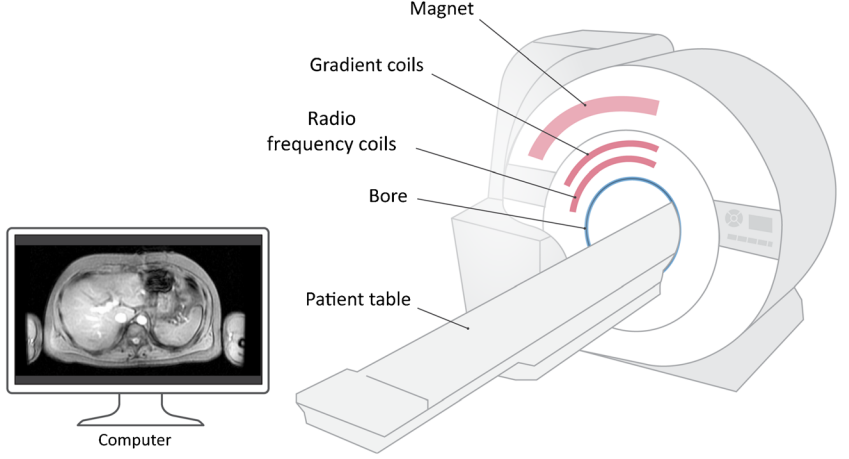
\includegraphics[width=\linewidth]{MRI-Schematic.png} 
 	\caption{Schematic of an MRI scanner taken from~\cite{Serai2021}.}
 	\label{fig:MRISchematic}
 \end{figure} 

\subsection{Magnetic Excitation and Relaxation} \label{SubSec:MagneticExcitationAndRelaxation}
%In the following section, the basic principles underlying MR imaging are presented. These include the relation between RF excitation and relaxation.
The base principles behind MR imaging are RF excitation and relaxation. Through these, the raw k-space data is measured which enable the reconstruction to an image. Terminology such as $T_1$ and $T_2$ relaxation times are introduced and explained. These are the basis for the pulse sequence discussed in section~\ref{SubSec:ImageAcquisitionAndK-Space}.

\subsubsection{Radio Frequency Excitation}
Individual nuclei precess around the field $B_0$ at a
resonance frequency known as the Larmor frequency $\omega_0$ of the net magnetization vector, which generally occurs in the RF range of the electromagnetic spectrum and is related to the external magnetic field as:
\begin{equation} \label{eq:LarmorFrequency}
	\omega_0 = \gamma \cdot B_0,
\end{equation}
with $\gamma$ being the gyromagnetic ratio, which is a fixed value depending on the nuclei~\cite{SamplingStrategies}. When nuclei are placed in the presence of a strong static magnetic field such as $B_0$ the nuclei split into two energy states, either aligned parallel to the magnetic field $B_0$ (called a spin-up state) or aligned anti-parallel to $B_0$ (called a spin-down state). The spin-up state has a slightly lower energy level as compared to the spin-down state and is therefore preferred. This slight difference in the spin states ($0.001\%$) results in an overall net magnetization $M$ aligned in the same direction as $B_0$. \\
To create an MR signal, the spins are excited out of their resting equilibrium, i.e. tipping $M$ away from $B_0$. To detect the signal from the hydrogen nuclei in the tissues an additional external field $B_1$ is introduced at the resonant Larmor frequency $\omega_0$ that can affect magnetization vector, causing it to rotate into a plane orthogonal to its original orientation. The rotated vector continues to precess around the $B_0$. The precession of the magnetization vector in the transverse plane can be detected by an RF coil tuned to the resonant frequency $\omega_0$. RF coils can be operated in a receive-only mode, in which case the inherent body coil is used as a transmitter; or the RF coils can be both transmit and receive. The purpose of the RF transmit coil is to create a time-varying $B_1$ field at right angles to $B_0$ that could be linearly or circularly polarized. The closer the receiving coil is to the source of the MR signal, the better the signal-to-noise ratio (SNR). Receiver coils generally comprise arrays of smaller individual coils or elements; however, each individual coil element has a limited depth penetration. \\
Multiple arrays of coils, termed phased-array coils, can be used together to achieve a higher coverage. The multiple coils are electronically decoupled from one another so that they do not appear as just a single large coil. The images from individual coils are independently reconstructed and then grouped together to create the final image. An RF pulse of amplitude $B_1$, called excitation pulse, is applied for a certain time duration to tip the magnetization at an angle away from the $B_0$ field. The precessing transverse magnetization induces a voltage in the receiver RF coil; this induced voltage is known as the free induction decay. After the pulse, the magnetization returns to thermal equilibrium by processes known as MR relaxation. To fully encode the spatial information within the field of view (FOV), pulse sequences must be iterated numerous times. The time between successive iterations of a pulse sequence is known as the repetition time (TR). The time between the application of the initial RF pulse and the middle of the detected echo is known as the echo time (TE). Due to this the overall time to acquire an MR image is quite long~\cite{Serai2021}.\\

\subsubsection{Magnetic Relaxation}
Once the RF pulse is turned off, $M$ continues to precess as it returns to its thermal equilibrium state. During this time, two types of relaxation occur: $\text{T}_1$ (longitudinal or spin lattice) and $\text{T}_2$ (transverse or spin/spin). One attribute that makes $\text{T}_1$ and $\text{T}_2$ so valuable for determining the signal in MRI is their sensitivity to the presence and type of tissue. It is this tissue dependence property that gives MR its excellent soft-tissue contrast. $\text{T}_1$ relaxation describes the recovery of the longitudinal magnetization back to thermal equilibrium following a perturbation by an RF pulse. The longitudinal component regrows along the Z direction with a time constant $\text{T}_1$. In other words, after the RF pulse is turned off, the protons that were disturbed give their energy to the surrounding environment and return back to their original equilibrium state, realigning with $B_0$. Hence, $\text{T}_1$ relaxation is also called longitudinal relaxation. Furthermore, because $\text{T}_1$ relaxation involves the loss of energy that was put into the spin system by the RF pulse, it is also referred to as spin-lattice relaxation, the lattice consisting of surrounding macromolecules. This loss of energy is stimulated by the fluctuating magnetic fields associated with the dipole–dipole interactions of neighboring magnetic moments. $\text{T}_1$ relaxation can only occur when these magnetic field fluctuations occur at the resonant frequency $\omega_0$. The rate at which the spin magnetization $M_z$ recovers to $M_0$ at time $t$ is called $\text{T}_1$ relaxation time. It can be expressed as follows:
\begin{equation}
	M_z = M_0 \cdot \bigg(1 - e^{-\frac{t}{\text{T}_1}} \bigg).
\end{equation}
A preferred method of measuring $\text{T}_1$ relaxation is the Look-Locker method, which is based on the principle that one does not need to wait for the net magnetization vector to equilibrate in order to measure $\text{T}_1$. Instead, an RF pulse is used with a small flip, which can be repeatedly applied. The acquisition pulse sequence is designed to generate a train of signals that gradually approaches a steady-state recovery. The recovery curve measured by this technique can be fitted to an exponential curve to provide an effective $\text{T}_1$ measurement. This has become one of the most popular $\text{T}_1$-mapping method for abdomen and cardiac imaging. The general principle of $\text{T}_1$ mapping is to acquire multiple images with different $\text{T}_1$ weightings and to fit the signal intensities of the images to the equation of $\text{T}_1$ relaxation. $\text{T}_1$ relaxation values for tissues can be estimated by fitting the data to the following equation:
\begin{equation}
	S = S_0 \cdot \bigg(1 - A \cdot e^{\frac{\text{TI}}{\text{T}_1}} \bigg),
\end{equation}
where $S$ is the signal intensity measured at each inversion time value $\text{TI}$, $S_0$ is the initial signal intensity at time $t=0$ and $A$ is
a constant.\\
$\text{T}_2$ relaxation results in the loss of transverse magnetization caused by interactions between the magnetic fields of neighboring hydrogen nuclei. It is not an energy loss process like $\text{T}_1$ but is a loss of phase coherence within the spin system. This process, also known as spin-spin relaxation, leads to the destruction of transverse magnetization and causes the magnetic moments of the tissue to dephase. $\text{T}_2$ mapping is a method of measuring the $\text{T}_2$ value of the tissue. $\text{T}_2$ relaxation time can be calculated using a $\text{T}_2$ sequence with different echo times (TEs). The most fundamental sequence for $\text{T}_2$ mapping is signal measured with spin echo techniques (multiple sequences with different TE values). Other 2-D sequences have been used, such as multi-echo spin echo (MSME) and fast spin echo (FSE). Synthetic MRI is another quantitative method in which a single saturation recovery turbo spin-echo sequence is used to estimate $\text{T}_2$ transverse relaxation. $\text{T}_2$ relaxation values for tissues can be estimated by fitting the data to the following equation using a mono-exponential decay curve:
\begin{equation}
	S(\text{TE}) = S_0 \cdot e^{\frac{\text{TI}}{\text{T}_2}},
\end{equation}
where $S(\text{TE})$ is the signal intensity measured at each $TE$ and
$S_0$ is the initial signal intensity at time $t=0$.

\subsection{Image Acquisition and the Concept of K-Space} \label{SubSec:ImageAcquisitionAndK-Space}
After discussing the physical mechanisms behind MRI, it is time to look at the actual process of acquiring the image as well as the concept of the k-space. 
%\subsection{Image Acquisition and Pulse Sequences}
The image contrast in MR imaging arises from tissues generating MR signals with different intensities due to their physical properties. Contrast weighting of the MR signal is obtained by the design of pulse sequences, which consist of repetitive trains of RF pulses. Two of the most common pulse sequences are gradient echo 
%(GE) 
and spin echo 
%(SE) 
sequences. %\\

\subsubsection{Gradient Echo Sequence}
In a gradient echo (GE) sequence, the free induction decay (FID) signal is manipulated by a bi-polar gradient. The excitation pulse tilts the magnetization by $\alpha$ degrees. For $\alpha = 90°$ the longitudinal magnetization is rotated in the transverse plane. The data is sampled during a gradient echo at time TE after the excitation pulse. This gradient echo is achieved by dephasing the spins with a negative gradient before they are rephased by an opposite gradient with opposite polarity to generate an echo. A schematic overview of the process can be seen in Figure~\ref{fig:GradientEcho}. \\
The pulse sequence is repeated a number of times to acquire the entire image. 
%The time between two excitation pulses is called the repetition time. 
Changing the TR, TE, and flip angles of a GE sequence influences the contrast weighting. $\text{T}^*_2$-weighted contrast can be achieved by using small flip angles and a long TE and moderate TR. By using large flip angles, a short TR and a short TE, a $\text{T}_1$-weighted signal can be acquired. Using small flip angles in combination with a long TR and a short TE generates proton density contrast~\cite{PulseSequences}.%\\

\begin{figure}[htpb]
	\centering
	\graphicspath{{images/}{\main/images/}}
	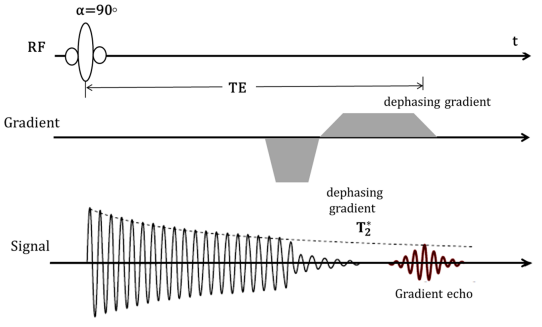
\includegraphics[width=\linewidth]{GradientEcho.png} 
	\caption{Schematic of an gradient echo sequence taken from~\cite{PulseSequences}.}
	\label{fig:GradientEcho}
\end{figure}

\subsubsection{Spin Echo Sequence}
With a spin echo (SE) sequence, pure $\text{T}_2$-weighted contrast can be generated. When a $90°$ pulse rotates the magnetization into the transverse plane, the resulting FID signal quickly decays due to the strong $\text{T}^*_2$ dephasing. If after a time $\frac{\text{TE}}{2}$ a $180°$ pulse is applied, the spins will be flipped and start to rephase. After another time, $\frac{\text{TE}}{2}$, a measurable echo signal is created. The spin dephasing due to static magnetic field inhomogeneities is compensated by inverting the spins with the $180°$ refocusing pulse. This process is visualized in Figure~\ref{fig:SpinEcho}.\\
Consequently, the decay of the signal at time TE will solely originate from the $\text{T}_2$ relaxation. A SE sequence can also be used to generate proton density or $\text{T}_1$-weighted signals by using a short TE and a long or short TR, respectively~\cite{PulseSequences}.

\begin{figure}[htpb]
	\centering
	\graphicspath{{images/}{\main/images/}}
	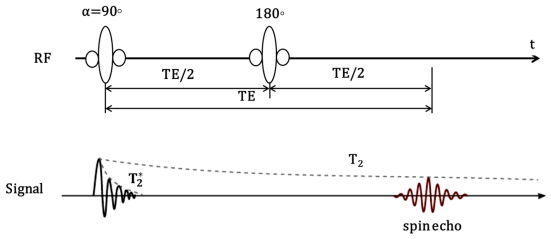
\includegraphics[width=\linewidth]{SpinEcho.png} 
	\caption{Schematic of an spin echo sequence taken from~\cite{PulseSequences}.}
	\label{fig:SpinEcho}
\end{figure}


\subsubsection{Introduction to K-Space}
The concept of the k-space is a generalization of the simple relation of a time-variant signal to a spectrum of two or more dimensions. An 2D image is related to a 2D k-space data set by a 2D FT, as seen in Figure~\ref{fig:2D_MRI_Measurement}
%, same as a 1D spectrum is related to the 1D signal by a normal (1D) FT. A 2D FT can be achieved by applying the (1D) FT successively row-by-row and column-by-column. 
As the FT is an information-preserving operation, the k-space data contains exactly the same information as the image data. Thus, in order to get the full image information, the full k-space data needs to be measured. The task of forming an image by this approach is then converted to the task of finding a way to measure the necessary corresponding k-space data. 
%An understanding of the physical meaning of the k-space domain can be derived from Figure~\ref{fig:1D_MRI_Measurement}. The time-domain signal defines the 1D k-space. Its coordinates are defined by the area under the gradient which the spins have experienced prior to the collection of each k-space data-point. 
Using the Larmor frequency again from Equation~\ref{eq:LarmorFrequency} the coordinates in 2D k-space will thus be given as $k_x = \gamma \cdot G_x \cdot t$ and $k_y = \gamma \cdot G_y \cdot t$. \\
In order to acquire an MR image, methods need to be developed 
%in order to get from one k-space point to the next. 
to traverse the k-space.
There are only two possibilities as seen in Figure~\ref{fig:kSpaceTrajectories}. The first one is to apply a gradient, in which case the k-space trajectory will be a line defined by the orientation of the gradient (see Figure~\ref{fig:constant_k-space_gradient}). As long as the gradient is kept constant, the k-space trajectory will be a straight line. 
%This way it is easy to see why simple superposition of two gradients will not produce an image. The resulting k-space trajectory will merely represent a straight line traversing k-space at some skewed angle. \\
The second method for traversing the k-space is the application of a refocusing pulse, which will lead to a jump of the k-space trajectory around the origin (see Figure~\ref{fig:refocusing_k-sapce_pulse}). It is clear that a spin-echo formation alone will not allow coverage of all of the k-space, since the trajectory would only jump between the two mirror symmetric points. A combination of spin echoes and gradients can, however, produce very efficient k-space trajectories. All of the existing k-space-based imaging techniques are based on some combination of these two basic means of traversing the k-space. \\
Is should be noted that the signals are measured 
%not continuously, but 
at discrete time intervals called the dwell-time of data acquisition. This discrete sampling leads to an ambiguous assignment of frequencies above a given threshold which is called the Nyquist frequency. The Nyquist frequency therefore determines the acquisition bandwidth inside which the signal should occur. The definition of the k-space coordinates implies that these are invariant with respect to the actual strength of the gradient used, as long as $G$ and $t$ are constant. Mathematically, data acquisition under a strong gradient and in a shorter acquisition time will yield the same k-space data and thus the same image as acquisition under a weaker gradient and a longer acquisition time. A shorter acquisition time and a closer spacing of sampling points are equivalent to a higher-acquisition bandwidth. Since the received noise grows with the square root of the bandwidth, a faster imaging technique will therefore by principle always carry the penalty of a lower signal-to-noise ratio (SNR)
%, even if all other factors influencing high-speed imaging are neglected. \\
For a conventional spin-echo imaging sequence
%, which is still widely used, 
a typical acquisition time of 5 to 10~ms for each phase-encoding step is used. Acquisition of 
%typically 
192 to 256 phase-encoding steps therefore requires a total net acquisition time of 1 to 2~s. However, this is much shorter than the 
%total 
actual
acquisition time of such a sequence, which is determined by the repetition time defined by the $\text{T}_1$-contrast. 
%From the aforementioned general considerations 
It 
%immediately 
follows that the SNR of a fast imaging sequence leading to acquisition times of approximately 50~ms, will be lowered by at least a factor of 5 to 10, regardless of the actual sequence used. 
%Fast imaging therefore requires improved SNR provided by radio-frequency coil designs. The improvement in SNR driven by the need for fast imaging will also benefit slower techniques, providing images with better spatial resolution and/or higher SNR. 
Fast imaging thus relies on radio-frequency coil designs improving the SNR.\\
The discrete data sampling has some additional consequences regarding the sampling density and coverage of data in k-space. Different parts of the k-space encode different features of the image: The center of the k-space hold the lower frequencies which represent the image contrast, whereas the outer parts encode the higher frequencies for sharp structures. Due to the symmetry of the 2D FT, this statement can also be reversed: The image center will be encoded by low-resolution k-space data. Therefore, sampling of sparsely distributed k-space data will reduce the effective field of view of the final image. \\
Mathematically, the final image will look exactly the same, irrespective of the way the data is sampled in the k-space. In practice, however, different approaches 
%to sampling 
can have a major impact on image quality
%. This is due to the fact that sampling 
as the data has to 
%proceed 
sampled
sequentially. The observed spins evolve not only as a function of the gradients defining the intended k-space trajectory, but are also influenced by other mechanisms unrelated to image encoding. It is noteworthy that the coordinates in k-space are expressed in units of a phase angle across space. Any mechanism affecting the phase of the signal along this trajectory will therefore alter the k-space trajectory. Some such commonly occurring mechanisms are flow and motion effects, magnetic field inhomogeneities, as well as susceptibility and chemical shift effects. The consequence of such phase effects in terms of imaging properties is dependent on the particular sequence and data sampling speed. In addition to phase effects, the signal decay with $\text{T}_2$ needs to be taken into account also, especially if the data acquisition time is similar or even longer than the $\text{T}_2$ of the observed tissues under construction~\cite{SamplingStrategies}.

\begin{figure}[h] %tpb
	\centering
	\graphicspath{{images/}{\main/images/}}
	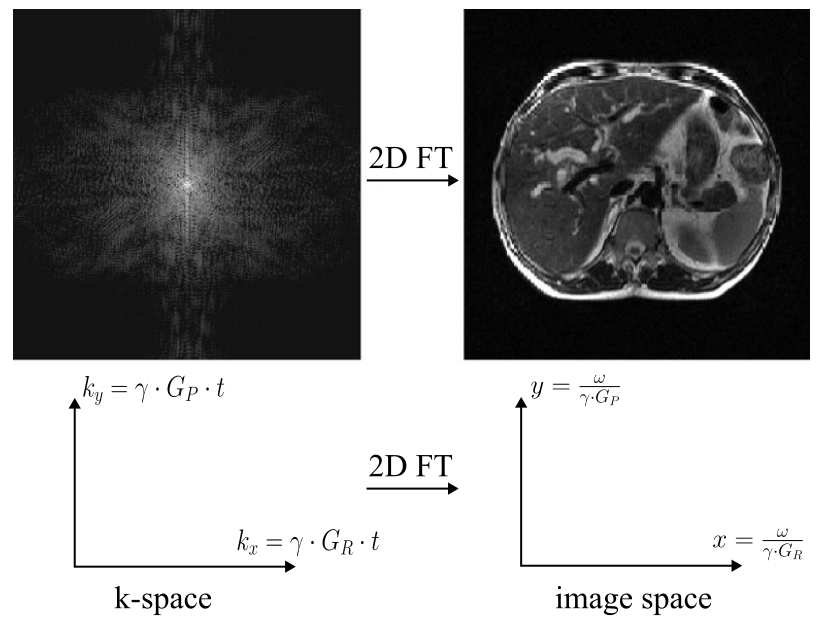
\includegraphics[width=\linewidth]{2D_MRI_Measurement.png} 
	\caption{Correspondence of the image domain and the k-space via a 2D FT, adapted from~\cite{SamplingStrategies}. The coordinates of each domain are defined by the Larmor frequency according to Equation~\ref{eq:LarmorFrequency}.}
	\label{fig:2D_MRI_Measurement}
\end{figure}

\begin{figure}[h] %tpb
	\centering
	\graphicspath{{images/}{\main/images/}}
	\begin{subfigure}{0.445\textwidth}
    		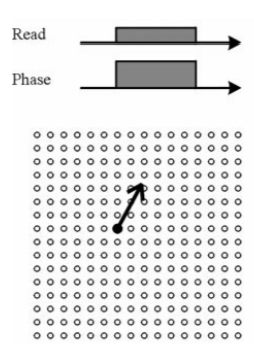
\includegraphics[width=\textwidth]{constant_k-space_gradient.png}
    		\caption{Schematic of a constant gradient creating a straight k-space trajectory.}
    		\label{fig:constant_k-space_gradient}
	\end{subfigure}
	\hfill
	\begin{subfigure}{0.445\textwidth}
    		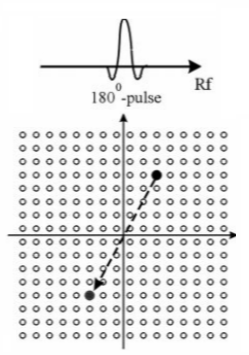
\includegraphics[width=\textwidth]{refocusing_k-sapce_pulse.png}
    		\caption{Schematic of an refocusing pulse inverting the phase of the k-space.}
    		\label{fig:refocusing_k-sapce_pulse}
	\end{subfigure}
	\caption{Methods of moving in the k-space using a) constant gradients to move along straight lines or b) mirror the k-space at the origin using a refocusing pulse. Adapted from~\cite{SamplingStrategies}.}
	\label{fig:kSpaceTrajectories}
\end{figure}

\subsubsection{Rectilinear K-Space Sampling}
Almost all MR imaging sequences 
%used in clinical routine presently 
are based on rectilinear k-space sampling, i. e., the sampling points 
%in k-space 
are placed on a rectangular grid. This 
ia also referred to as Cartesian sampling and 
%reflects the ability to use a 
allows the usage of the fast Fourier transform (FFT) 
%for such a sampling strategy. It allows 
which enables 
image reconstruction in 
%considerably under 1~s
a very short time (under 1~s). 
%With special reconstruction processors, the reconstruction speed can be as high as 10 to 25 images per second. 
For comparison, using
the 
%general 
2D FT 
to transform a non-rectilinear grid can take about
%for transformation of a comparable number of non-rectilinear grid points in comparison requires
5 to 50~min per image~\cite{SamplingStrategies}.
%, using identical computer hardware. \\
In a Cartesian acquisition, one or more lines of k-space parallel to a Cartesian axis are collected following application of an RF pulse and generation of an RF echo. Adjacent points in a single line are collected in rapid succession in a single echo. The time between echoes and adjacent lines is much slower. The direction of fast acquisition is known as the frequency direction and the other one or two directions are known as the phase-encode direction or directions. Following line-by-line filling of k-space in a Cartesian sequence, each layer of a filled grid is subsequently used to reconstruct a single image slice~\cite{Bardo2021}.

%%% Old from Henning (to detailed....)
%Utilizing the two means of traversing the k-space, 
%%the basic techniques for 
%rectilinear sampling can be divided into spin-echo-based techniques and gradient-echo-based techniques. In all rectilinear sampling techniques, the gradient which is used during signal acquisition is commonly called the readout gradient, whereas gradients used to bring the k-space trajectory to a certain starting point before data acquisition are called phase-encoding gradients. \\
%A gradient echo is formed using a reversal of the readout gradient. In conventional gradient-echo imaging, only the refocusing part of the k-space trajectory is measured, whereas the signal dephasing as well as phase encoding is performed prior to data acquisition (Fig. 8). The experiment is repeated after the recovery time TR, using different offsets of the phase-encoding gradient prior to each acquisition step. Using the k-space, it can be easily seen how gradient-echo imaging can be generalized to a faster technique, using less excitation periods by sampling more than one k-space line after each excitation. Repeating gradient reversal and the application of a phase-encoding gradient can be used to read out several k-lines per acquisition with a concordant reduction in total imaging time. In the extreme case, all k-space data can be read out following a single excitation. This is called the single-shot, echo-planar imaging (EPI) sequence~\cite{EPI}. \\
%%Historically, the development took place the other way round: EPI was first invented by P. Mansfield, and gradient echoes followed several years later. The concept of the k-space was not widely known at that time, therefore, the intrinsic relationship between the two techniques has only been acknowledged gradually. 
%Despite the close conceptional similarity between EPI and gradient echo techniques
%%with respect to their k-space trajectories
%, both types of sequences have vastly different imaging and hardware implications. This difference is caused by the sequential sampling of k-space points and the resulting influences on the signal of the mechanisms mentioned previously. As the signal decays with $\text{T}_2$ the signal amplitude is reduced during data acquisition. For conventional gradient-echo imaging, even with moderate gradient strength (and thus longer acquisition times), this effect is inconsequential since the typical acquisition times of 5 to 10~ms are considerably shorter than the typical $\text{T}_2$ of tissues. For EPI, however, the total acquisition time for n k-space lines is n times longer, even if the time necessary for gradient reversal and phase encoding is neglected. For the moderate acquisition times noted previously, this will lead to total acquisition times of 1~s or more, which exceeds most $\text{T}_2$ values observed in human tissues. 
%%Dephasing of spins across the selected slice will lead to $\text{T}_2$ of the order of 100~ms at most. 
%For identical acquisition times, as in our gradient-echo example, the signal will have vanished long before the end of data acquisition leading to information loss. 
%%Depending on whether data acquisition has commenced at the center or in the outskirts of k-space, the resulting image will either be severely blurred or reveal merely contours without contrast. This illustrates that 
%Thus EPI 
%%absolutely 
%requires very fast data acquisition in order to 
%%acquire 
%scan all of the k-space data within 
%%not much more than 100~ms at most; otherwise, 
%100~ms or else image quality will deteriorate significantly. In the given time range, state-of-the-art scanners can acquire 64 to 128 phase-encoding steps. Longer acquisition times allowing for higher 
%%nominal 
%resolution are of course technically feasible, but the $\text{T}_2$-decay 
%%of the signal will 
%prohibits the realization of this 
%%nominal 
%resolution. 
%%Since cerebral spinal fluid (CSF) has a long $\text{T}_2$, EPI images of the head with long acquisition times can look deceptively sharp. It must be noted, however, that the perceived sharpness applies only to CSF-filled structures, whereas the true resolution of parenchyma with a $\text{T}_2$ of approximately 60~ms is considerably worse. 
%With even stronger and faster gradients it is 
%%of course feasible 
%possible to acquire true high-resolution images with short acquisition times, but the penalty in SNR for such applications is too severe and has prohibited its use for most forms of morphological imaging. The EPI technique has emerged, however, as an ideal vehicle for functional imaging either in BOLD-based fMRI, in first-pass perfusion measurements or in diffusion imaging, but it is not a viable technique for high-resolution morphological imaging~\cite{SamplingStrategies}.\\
%Even for short acquisition times, EPI suffers from severe problems regarding its imaging properties, which are caused by the phase-altering mechanisms mentioned previously. Chemical shift effects and susceptibility both lead to signal phase shifts which increase linearly with time. Since data acquisition along the readout gradient is fast, there is little effect in the readout direction. In the phase-encoding direction, however, the dwell time amounts to the acquisition time of one k-space line. 
%%For the acquisition of 64 k-space lines in 64~ms, the field of view in frequency units will be 1000~Hz. For a frequency shift of fat vs water of approximately 200~Hz at 1.5~T, this will mean that the signal of fatty tissue will be shifted by 20$\%$ of the image width. The resulting misregistration artifact necessitates the use of fat suppression for practically all EPI applications. 
%Field inhomogeneity and susceptibility will lead to a similar shift. Since the resulting frequency shifts are not as discrete as chemical shift effects, the misregistration will vary continuously leading to highly non-linear image deformations. An additional problem in EPI relates to the fact that the k-space trajectory runs in opposite directions in every other k-space line due to the alternating polarity of the readout gradient. Any asymmetry in the acquired data will therefore lead to some slight perturbation in any other line known as the $180°$ artifact.  
%%The final image will therefore be a superposition of the true image with an image representing the perturbation in every other k-space line. From this discussion of the k-space trajectory, it is easy to see that this perturbation will generate an image which is displaced by half the field of view in the phase-encoding direction. This is the so-called $180°$ artifact.
%\\All the confounding factors discussed will produce such artifact. With appropriate post-processing routines based on reference signals, some of the sources of artifacts can be corrected for. In general, the $180°$ ghost will become stronger whenever any of the mechanisms mentioned previously become significant and will therefore deteriorate the image quality further. Motion can also cause phase-effects on the signal. With an alternating readout gradient, motion along this direction will be refocused in every even refocusing period. Consequently, a flow-dependent $180°$ ghost will occur. Motion along the phase-encoding direction will lead to a velocity-dependent increase in the signal phase and consequently to a velocity-dependent signal displacement. 
%%Signal from a round vessel with laminar flow will therefore appear as a boomerang-shaped artifact displaced from the vessel wall. Any vascular diagnosis based on EPI images therefore has to be made with the utmost care. The inherent artifact behavior limits the practical use of EPI to examinations of the head. Abdominal or thoracic EPI and even cardiac EPI have not been developed beyond a feasibility state. They require considerable efforts in region-selective shimming and even post-processing, using actual field maps of the patient such that the time advantage of EPI is lost. 
%Thus, for the time being, EPI 
%%therefore has to be
%is regarded as a brain-only technique 
%%where it serves as a vehicle for the 
%for fMRI applications, including diffusion and perfusion imaging~\cite{SamplingStrategies}.\\
%Conventional gradient-echo imaging suffers from no such effects and can therefore be applied all over the body with no or only mild susceptibility misregistration. Chemical shift effects will, however, influence the contrast of gradient-echo images by the chemical-shift-dependent dephasing of fat and water signals. Signals from fat and water protons located at the same position will periodically be in- and out of phase with each other in a time interval determined by their difference in Larmor frequencies. 
%%For 1.5~T the time difference between the two extreme conditions will be approximately 2.5~ms. Images acquired with TEs differing by 2.5~ms will look dramatically different due to this effect, although $\text{T}_2$-dependent effects for such small TE differences will be negligible. 
%As shown in Fig. 11, the out-of phase image will show a considerable reduction in signal amplitude in tissues containing both fat and water protons such as bone marrow. In addition, an artificial black line will appear at the interface between fatty and water tissues due to the zero crossing of the signal between these antiphasic images. When (im)properly used, this artifact can be used to beautify images, giving them a crisp and well-defined appearance. Care must be taken, however, not to mis-read this artifact as an anatomical structure. With respect to the total acquisition time, gradient-echo imaging is somewhat slower than EPI due to the necessity of repetitive application of excitation pulses. Gradient-echo sequences, which are optimized for speed, typically achieve imaging times of 200 to 400~ms, using gradient systems comparable to those of EPI. Due to the strong signal saturation caused by the very short repetition times, the intrinsic SNR is comparably low. \\
%%(but for many applications still satisfactory). 
%%The SNR can be optimized by using low-excitation flip angles and/or total signal refocusing (true FISP). In combination with bolus application of contrast agent, gradient-echo sequences allow the acquisition of MR angiograms especially of the thorax, abdomen, and the extremities with unprecedented image quality. This  relatively new application has led to whole new field of applications for gradient-echo imaging. \\
%In order to reach a compromise between the more efficient sampling of EPI and the much more benign artifact behavior of gradient echoes, 
%%segmented 
%mixed approaches have been developed. In these approaches, more than one excitation is used and several k-lines are sampled per excitation. 
%%Depending more on the perspective of their creators than on anything else, such approaches are called multi-echo gradient echo, multi-shot EPI, or segmented EPI. 
%The optimum number of k-lines per excitation is strongly dependent on the particular application
%%; it 
%and can range from 3 for MR angiography and cardiac imaging to 64 or more for high-resolution head imaging.

%\subsection{Spin-Echo Techniques}
%In spin-echo techniques, refocusing pulses are used in the construction of the k-space trajectory. Conventional spin-echo techniques acquiring one k-line per excitation are identical to gradient-echo techniques with respect to the k-space sampling strategy used. In rapid acquisition relation enhanced imaging (RARE, e. g., turbo spin echo and fast spin echo), multiple refocusing pulses are employed in order to sample more than one and, in the extreme case, all k-lines per excitation [15]. In order to suppress unwanted coherences, the k-space trajectory in RARE has to be brought to the identical position at the time of application of each refocusing pulse. This is achieved by using a phase-encoding rewinder after reading out each k-line (Fig. 12). Conceptionally, RARE is very similar to EPI, however,
%%and the possibility to build a spin-echo-based technique has already been mentioned in the original paper by Mansfield. 
%The spin-echo refocusing makes a huge difference with respect to the artifact behavior. For once it should be noted that the direction of data sampling is identical for all k-lines. Therefore, no $180°$ ghosts will occur. In addition, all phase changes caused by chemical shift, susceptibility, etc., are refocused. The phase effects therefore do not accumulate but re-start in each k-line just like in conventional spin-echo sequences. Motion effects are in principle similar to the ones discussed for EPI with a refocusing of flow in every even echo. Since for low flow the resulting $180°$ effect will be weak, and for high-flow velocity the signal will vanish from the image due to outflow during the echo train, the resulting flow artifact behavior of RARE is very benign. 
%%Slow-flow vessels (e. g. liver veins), which are black on conventional spin-echo imaging, appear very bright on $\text{T}_2$-weighted RARE imaging due to this even echo refocusing effect.
%The insensitivity to other mechanisms leads to $\text{T}_1$ and $\text{T}_2$ as the basic contrast mechanism for RARE. From the discussion of the properties of k-space it follows that the $\text{T}_2$-contrast is determined by the echo times of the acquisition of the k-lines with low phase encoding. The $\text{T}_2$-contrast of a given implementation can thus be varied widely by changing the order of the phase-encoding gradient. By similar consideration, $\text{T}_2$-relaxation along the echo train leads to a loss of resolution when the k-lines carrying the edge information are acquired at long echo times. For most diagnostic applications in high-resolution imaging, a segmented acquisition is therefore preferred with echo train lengths ranging between 8 and 35 for $\text{T}_2$-weighted scans and 3 to 5 for $\text{T}_1$-weighted scans. Nevertheless, single-shot variants are also being used~\cite{SamplingStrategies}. 
%%Especially single-shot RARE (or single-shot FSE) with very strong $\text{T}_2$-contrast has been shown to be extremely useful for imaging of liquid-filled structures like in MR myelography [16], MR urography [17], or MR cholangio-pancreatography (MRCP) [18]. 
%Using half-Fourier phase encoding in half-Fourier acquired single-shot turbo spin echo (HASTE) [19], single-shot implementations with less $\text{T}_2$-contrast are also feasible. It has been noted that signal from fat is significantly brighter in RARE compared with conventional spin-echo imaging at equal echo times [20]. This is due to so-called J coupling of protons in lipids, which leads to a periodic modulation of their resonances just like the modulations caused by two elastically coupled pendulums [21]. This modulation will not be refocused but continue despite the reversal of the phase by the 180 pulse (Fig. 13). At a time interval equal to 1/(2 J), the signals from such coupled spins will be opposed and therefore canceled. For typical coupling constants, this condition is reached at echo times of 80 to 140 ms typically used for $\text{T}_2$-weighted imaging. The multiple refocusing in an echo train ensures that the phase of the signals from coupled spins stay together along the echo train; thereby, signal suppression is avoided and fat will appear bright. A similar cause is implied for a relative reduction in susceptibility contrast on RARE images (Fig. 14). Static susceptibility effect will be refocused on both spin-echo sequences. If spins move along strong local gradients as caused by hemorrhage, for example, the motion-dependent variation of their Larmor frequency cannot be refocused due to the random nature of the motion. Multiple refocusing pulses, however, will ensure that the spin phases stay together. Some such diffusion-dependent dynamic susceptibility effect is observed in most organs (nuclei in the brain and basal ganglia, liver, lung, etc.). Therefore, RARE images can look very different from conventional spin-echo images at identical echo times. Due to the repetitive use of refocusing pulses and the necessity for rewinding the phase-encoding gradient, RARE is inherently slower than EPI. The gradient performance of current scanners allows refocusing intervals as short as 4 ms or less. The high radio-frequency power inherent to a long train of $180°$ pulses limits, however, the range of applications for such fast echo trains. Even though this problem can be ameliorated by the use of lower refocusing flip angles, EPI with typical readout times of 1 ms or less will remain faster. The big advantage of spin-echo techniques remains, however, their lack of distorting artifacts which makes spin-echo techniques applicable all over the body. Even high-quality cardiac images with HASTE have been demonstrated as well as perfusion and ventilation imaging of the lung [22].

\subsubsection{Non-Rectilinear K-Space Sampling}
A common problem of rectilinear sampling techniques is the very heterogeneous nature of the k-space trajectories used: Data are acquired along straight k-space lines under a constant gradient. Going around the corner of the trajectory requires very fast switching for a brief period. 
This 
%The combination of both modes of operation 
is very demanding on the gradient power amplifiers, which have to be able to alternate between the two modes. A more common load on the gradients is offered by the use of curved k-space trajectories. Especially spiral trajectories~\cite{SpiralMRI, SpiralMRI2} have won considerable interest due to their very efficient use of the gradient system. 
%For a given gradient system it is also possible to calculate the trajectory achieved by running the gradient system always under full load. In terms of the gradient performance, spirals therefore are considerably more efficient than rectilinear k-space trajectories. 
A practical problem relates to image reconstruction which requires algorithms not (yet) commonly available and which can take several seconds per image on a typical scanner~\cite{SamplingStrategies}. 
%In order to make use of the very fast FFT algorithm, the typical approach to reconstruction of data sets acquired with spiral (or other non-rectilinear) trajectories is to first interpolate the data onto a rectilinear grid and then to use FFT for the reconstruction itself. With further developments of spirals, it is expected that reconstruction algorithms will become widely available. 
The ultimate success of spiral imaging will then be determined by its inherent imaging properties, which are significantly different from rectilinear scans. Constant off-resonance effects, such as chemical shift, field inhomogeneity, and susceptibility, will not lead to a displacement in the phase-encoding direction, but to blurring of the corresponding structures~\cite{SamplingStrategies}.
%Firstly, it should be noted that spirals do not have a preferred orientation like the readout- and phase-encoding direction in rectilinear scans. Constant off-resonance effects, such as chemical shift, field inhomogeneity, and susceptibility, will therefore not lead to a displacement in the phase-encoding direction. It will instead lead to blurring of the corresponding structures~\cite{SamplingStrategies}. 
%In some respects this can be regarded as an advantage since the severe distortions of EPI images are avoided. On the other hand, some mild distortion in EPI images can be tolerable for most applications, whereas blurring artifacts are not. \\
%These artifacts can be avoided if the off-resonance frequency is known. The data can then be corrected and a sharp image will be produced. Consequently, for most applications of spiral imaging a field map is acquired prior to the scan in order to measure the local off-resonance effects. 
A problem of spiral imaging is the fact that severe artifacts can arise when the k-space trajectory produced by the gradient system is not exactly identical to the trajectory used for image reconstruction. It is thus necessary to accurately calibrate the gradient system or to even measure the actual trajectory used. 
%Especially spiral images in tilted orientations involving all gradients simultaneously sets very high requirements for the gradient switching behavior. 
A favorable property of spirals is the motion correction inherent to the trajectory~\cite{SpiralMRI3}. 
%The periodic nature of spirals ensures that part of the data are motion corrected. For the remainder, motion-dependent dephasing will be mild. Consequently, spirals have been demonstrated to yield good image quality for moving structures like blood in vessels or even the heart. It is noted that EPI also has an inherent motion correction in every even refocusing period, as discussed previously. The interleaved nature of motion-corrected and motion sensitized k-lines leads, however, to a 180 artifact, whereas in spirals the distribution of motion-corrected and motion-sensitized data is continuous and therefore no artifacts are formed. 
Apart from spirals, other non-rectilinear k-space trajectories have been suggested. 
%Back projection uses a star-like trajectory and was in fact the method used by Lauterbur [27] in his first demonstration of MR imaging. 
Back projection uses a star-like trajectory and allows the realization of extremely short echo times 
%and has therefore found applications especially for imaging of solid structures. 
Its inhomogeneous k-space coverage with a high sampling density for points at the center of k-space and its somewhat awkward artifact behavior have limited its success for conventional imaging~\cite{SamplingStrategies}. \\
%Folgenden Teil rausnehmen?
Other trajectories, such as rosettes or even random k-space trajectories, have also been explored. A common feature of all non-rectilinear trajectories relates to their non-periodic nature, which produces severe artifacts when the field of view of the data acquisition is less than the size of the object. For rectilinear scans this leads to severe fold-over artifact, which can be tolerated as long as it does not affect relevant structures or even is totally avoided when it occurs in the readout direction, where oversampling can be applied without penalty in the data acquisition time. For non-rectilinear scans oversampling is not an option, since the field of view is determined by the distance between adjacent parts of the trajectory, rather than by the sampling rate along the trajectory. 
%Oversampling therefore requires a denser k-space trajectory with concordant prolongation of the acquisition time. 
For an insufficient field of view of the k-space data, misregistration artifacts can be very severe, depending on the trajectory used. Spirals produce a circular rim artifact around the image. It is therefore mandatory to ensure that the k-space trajectory is sufficiently dense to always cover the whole object of interest~\cite{SamplingStrategies}. 
%This limitation is especially severe for cardiac imaging, where the size of the field of view of a short axis plane can be considerable. Limitation of the field of view by the use of surface coils with limited sensitivity range is therefore mandatory for many applications of non-rectilinear trajectories.

\subsection{Imaging Acceleration and Reconstruction} \label{SubSec:ImagingAccelerationReconstruction}
To alleviate the slow image acquisition times of the MR imaging, different MRI acceleration techniques are used. Most of these included scanning less k-space lines during signal acquisition, omitting certain frequencies by zero-padding.
%higher frequencies and fully scanning the center region. 
The amount of k-space lines that are zeroed out are usually given by a reduction factor $R$. While there are different subsampling techniques, most involve fully sampling a center region containing the lower frequencies and dropping higher frequencies. These are deemed less important as they contain mostly details and fine image structures, whereas the low frequencies encode the general image structure and contrast. All of these methods create artifacts, like image blur, during image reconstruction, as seen in Figure~\ref{fig:ExamplesSubsampling}. In order to still reconstruct images with as few artifacts as possible, different technologies have been developed such as parallel imaging and compressed sensing, which are discussed in the following sections.

\begin{figure}[htpb]
	\centering
	\graphicspath{{images/}{\main/images/}}
	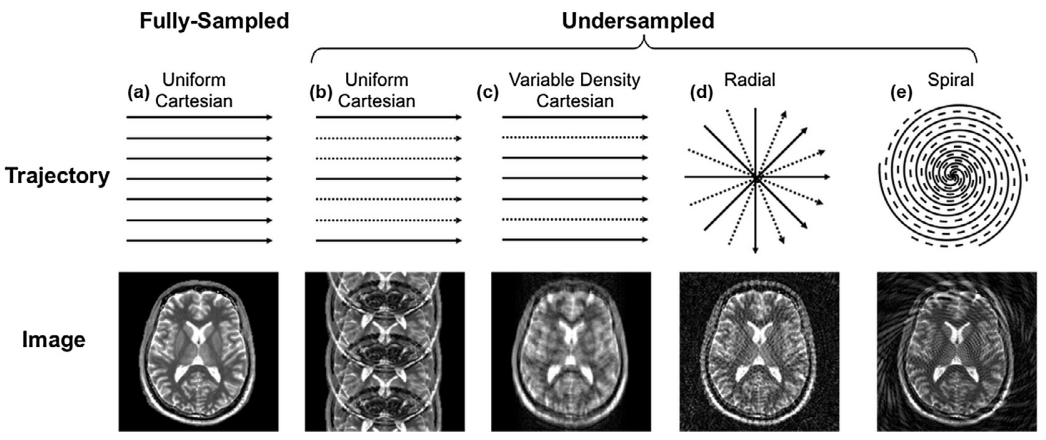
\includegraphics[width=\linewidth]{ExamplesSubsampling.png} 
	\caption{Examples of different subsampled k-space trajectories and their associated aliasing artifacts (omitted/zeroed data represented by dashed lines) taken from~\cite{AdvancesPI}.}
	\label{fig:ExamplesSubsampling}
\end{figure}

\subsubsection{Parallel Imaging}
Parallel imaging (PI) is a robust method for accelerating the acquisition of MRI data by subsampling the k-space data using an array of receiver coils. One of several PI algorithms can then be used to reconstruct artifact-free images from either the aliased images (SENSE-type reconstruction) or from the under-sampled data (GRAPPA-type reconstruction). PI requires special hardware known as phased array coils that 
%are now supplied with nearly every modern clinical scanner. Phased arrays 
contain multiple independent receiver channels. Each coil element is most sensitive to the magnetization closest to it and less sensitive to magnetization further away. 
%The spatial sensitivity can be visualized as the coil’s sensitivity profile (Fig. 3). Note that in these maps, the coil sensitivity falls off rapidly with increasing distance from the coil. 
Individually, each coil has high local signal-to-noise ratio (SNR) but inhomogeneous coverage. To expand the FOV while maintaining high SNR, several coils are organized in an array. The images from each channel are usually combined into a single image with relatively homogeneous intensity by taking e.g. a root sum-of-squares combination.
% or using more advanced methods that preserve SNR [14]. Dedicated surface coil arrays are provided for different parts of the body. Coil arrays can have up to 32 [15,16], 64 [17], or 96 [18] channels for brain imaging or 128 channels for cardiac imaging [19], although most high-count arrays are still in research development.
%Intuitively, every coil can be used to generate a unique view of the object, which provides additional spatial information that can partially replace gradient encoding to reduce scan time. Each coil detects signals from the object weighted by the coil’s sensitivity profile. This weighting can be modeled as a multiplication of the coil sensitivity profile and the magnetization. The use of a coil with an inhomogeneous sensitivity also affects k-space. Multiplication in the image domain is equivalent to convolution in the frequency domain. Therefore, in k-space the Fourier Transform of the image is convolved with the spectrum of each coil’s sensitivity profile.
Theoretically, the maximum acceleration factor is limited by the number of coils
%, as will be explained in the SENSE section. 
,thus, for PI to be successful, each coil must have a unique sensitivity variation along the direction that is accelerated. For example, an array with four coils arranged in a line may be able to attain a maximum R = 4 along one direction, but no acceleration would be possible in the perpendicular direction~\cite{AdvancesPI}.\\
As mentioned before, PI techniques fall into one of two classes, depending on whether aliased pixels are separated in the image domain (SENSE) or missing phase encoding lines are reconstructed in k-space (GRAPPA). Sensitivity encoding (SENSE)~\cite{SENSE1} is a PI technique which unfolds superimposed pixels in the image domain. For Cartesian k-space sampling with a uniform acceleration factor of R = 3 and a receiver array with four coils the undersampling reduces the FOV threefold, such that three pixels from the fully-sampled image fold onto the same pixel in the aliased image. SENSE uses prior knowledge of the coil sensitivity profiles to separate folded pixels and recover the full FOV image. 
%The first step in the SENSE reconstruction is to form a sensitivity matrix S for a given pixel in the aliased image. This matrix has size nc  np, where nC is the number of coils and np is the number of aliased pixels, which is equal to the acceleration factor. Let the signal at location ðx; yÞ in the aliased dataset received by coil j be denoted I aliased j ðx; yÞ. It can be expressed as the sum of three pixels in the full FOV image that have been weighted by their coil sensitivities and are separated by distance FOV=3.
If the acceleration factor exceeds the number of coils, then the
SENSE 
%equations will not be invertible. 
algortihm will not be able to recover an un-aliased image.
In practice, the largest achievable acceleration factor is usually smaller than the theoretical limit because coil sensitivities overlap and are not orthogonal~\cite{AdvancesPI}.\\
One common feature of PI is the amplification of noise in the reconstructed image, though with varying degrees:
\begin{equation} \label{eq:SNR-SENSE}
	SNR_{SENSE}(x,y) = \frac{SNR_{full}(x,y)}{\sqrt{R} \cdot g(x,y)},
\end{equation}
where the geometry factor $g(x,y)$ describes the spatial pattern of noise enhancement, $SNR_{SENSE}(x,y)$ the SNR in the reconstructed SENSE image and $SNR_{full}(x,y)$ the SNR of the fully sampled image. In addition to the g-factor losses, which depend on variables like number of coils, array configuration, etc., the SNR decreases with the square root of the acceleration factor $R$, which is known as Fourier averaging.\\
%It depends on many variables, including the number of coils, array configuration, coil loading, and scan plane orientation. The signal-to-noise ratio (SNR) in the reconstructed SENSE image is related to that of the fully sampled image according to
While SENSE unfolds aliased signals in the image domain, generalized partially parallel acquisitions (GRAPPA)~\cite{GRAPPA} synthesizes missing data points directly in k-space. 
%As described above and shown in Fig. 3, collecting data with multiple inhomogeneous receiver coils weights the magnetization by each coil’s sensitivity profile. In k-space
There, the use of inhomogeneous receiver coils effectively spreads information from one k-space point to nearby k-space points. GRAPPA exploits these k-space redundancies across coils to reconstruct missing k-space data using neighboring acquired points. A single missing k-space data point (target point) is synthesized as a linear combination of acquired neighboring k-space points (source points) with the spatial arrangement of source and target points being called GRAPPA kernel. Each acquired source point is multiplied by a coefficient (GRAPPA weight) and the results are added to estimate the target point. A single target point for one coil is reconstructed using source points from all other coils. For Cartesian sampling, the weights are shift invariant to a first approximation, so the same GRAPPA weights can be applied throughout k-space. The reconstruction can be described as convolving or sliding the GRAPPA kernel throughout k-space.
%; as the kernel moves from point to point, the weights are multiplied by the kernel source points to reconstruct the kernel’s target points (Fig. 7). A typical kernel may consist of six source points from each coil, with three in the readout direction and two in the phase encoding direction, centered around a target point. Including more source points tends to improve the reconstruction quality but may require additional calibration data, as discussed below.
While SENSE uses additional information in the form of coil sensitivity profiles to unfold aliased pixels, GRAPPA requires extra data to estimate the weights. GRAPPA is considered to be autocalibrating because several additional phase encoding lines, called the auto-calibration signal (ACS), are collected near the k-space origin for calculating the weights. 
%The GRAPPA kernel is moved to every possible position within the ACS to accumulate many instances where the source points and target points are both known. Then the GRAPPA equation can be inverted to solve for the unknown weights.
The SNR of images reconstructed using GRAPPA is also reduced according to Equation~\ref{eq:SNR-SENSE}, however, because GRAPPA does not require an explicit estimate of the coil sensitivities, it tends to be more robust than SENSE to inconsistencies between the calibration and undersampled data~\cite{AdvancesPI}.\\
SENSE and GRAPPA can be combined in what is called iterative self-consistent parallel imaging (SPIRiT)~\cite{SPIRiT}. Like GRAPPA k-space kernels are used to recover missing information by exploiting correlations between neighboring k-space points, though the reconstruction is framed as an inverse problem similar to SENSE. Regardless of the original sampling trajectory, SPIRiT outputs a Cartesian k-space. The reconstruction is typically initialized with the undersampled zero-filled k-space and is solved iteratively. 
%as an optimization problem. 
%On each iteration, the algorithm moves toward a solution that 
The algorithm 
minimizes and balances the errors of two terms: calibration consistency and data consistency. The first is calculated using a so-called SPIRiT kernel in the k-space similar to GRAPPA, while the second term enforces consistency with the undersampled data as the difference between the reconstructed data and acquired data should be zero at the originally sampled positions. Thus reconstruction should only recover missing k-space points without changing the known data points~\cite{AdvancesPI}.%\\
ESPIRiT~\cite{ESPIRiT} is an extension of SPIRiT that uses k-space kernel operations to derive a set of eigenvector maps that behave like coil sensitivities, which can be incorporated in a generalized SENSE reconstruction. This requires calibration data from the fully sampled region at the center of k-space. 
%A k-space kernel is moved to each possible position within this region, and each instance of the kernel is reshaped to populate a row in a special matrix. Many of the singular values of this matrix are small or close to zero, meaning that it has a null space. The existence of a null space implies that neighboring k-space points in the multichannel data are correlated. Missing k-space data are reconstructed by recognizing that this relationship should be true not only over the calibration region but also over the entire k-space.
Unlike SENSE and GRAPPA, SPIRiT reconstructs images iteratively and can require long computation times which can be addressed by using e.g. parallelized GPUs~\cite{AdvancesPI}.

\subsubsection{Compressed Sensing}
The idea behind compressed sensing (CS) is that sparse or compressible signals can be acquired in an efficient way by applying compression already in the data acquisition process. According to CS theory, sparse or compressible signals can be recovered from fewer samples than required by the Shannon-Nyquist sampling theorem~\cite{CS-MRI}. This is achieved by applying an appropriate sampling scheme and reconstruction that employs signal sparsity to recover the signal. MRI fulfills two important requirements for the application of CS: medical imaging is naturally compressible by sparse coding and MRI scanners acquire samples of the encoded image in spatial frequency, rather than direct pixel values. CS emerged as an abstract mathematical idea that if one measures a relatively small number of random linear combinations of the signal values the signal can be reconstructed with good accuracy from these few measurements by a non-linear procedure due to the underlying signal being compressible.
% – much smaller than the number of signal samples nominally defining it. However, because the underlying signal is compressible, the nominal number of signal samples is a gross over-estimate of the effective number of degrees of freedom of the signal. As a result, the signal can be reconstructed with good accuracy from relatively few measurements by a non-linear procedure. 
In MRI, the sampled linear combinations are the individual Fourier coefficients (k-space samples) and CS is able to make accurate reconstructions from a small subset of k-space, rather than an entire k-space grid~\cite{CS-MRI}. It should be noted that unlike PI approaches, the k-space is incoherently sampled; thus, noise-like artefacts appear in the image when a direct inverse Fourier transform is performed. To remove the artefacts caused by the undersampling, iterative reconstruction is used. There are a number of sparsifying transforms that can be used for CS such as wavelets, which are very common, and total variation, which enforces the sparsity of the image gradients. The advantages of total variation include its simplicity, rotation invariance, and capability of preserving edges and providing good image quality~\cite{PulseSequences}. There are also several methods combining CS and PI trying to achieve higher acceleration factors~\cite{PI+CS, PI+CS2}.
%, but with the addition of regularization that enforces sparsity by penalizing coefficients in some domain (e.g. Wavelet, finite difference) with a $L_1$-norm

\subsubsection{Deep Learning Based Subsampling} \label{SubSubSec:DeepLearningBasedSubsampling}
There are also approaches for learning new subsampling strategies in a data-driven manner (pruning unimportant k-space frequencies)~\cite{MRISubsamplingPruning} as well as deep learning based radial~\cite{DeepMRIReconstructionRadialSubsampling} and non-Cartesian~\cite{DeepMRIReconstructionSubsampling} subsampling for MRI acceleration.


\subsection{Motion-Compensated Image Reconstruction} \label{SubSec:Motion-CompensatedReconstruction}
Patient motion during acquisition is one of the major impediments of high-quality MRI scans. This is especially true for thoracic and abdominal imaging, as organs move during breathing. Steps can be taken during or after the reconstruction to mitigate motion artifacts.

\subsubsection{Intraview and Interview Motion} \label{SubSubSec:IntraviewandInterviewMotion}
Due to the long acquisition times, motion is one of the major extrinsic factors influencing MR image quality. Patient and physiological motion induces aliasing along the phase-encoding direction and/or blurring of the image content~\cite{Kuestner2022}.
%, where the appearance depends on the imaging trajectory.
This motion can induce several consequences on MR signal formation. Intraview and interview motion have to be distinguished between: motion is intraview when occurring during individual MR experiments (between RF excitation and echo formation), whereas motion is interview when occurring between individual MR experiments. Whenever the period of motion is slow compared to the period of MR acquisition 
%defined by the repetition time 
$TR$, the assumption can be made that motion is interview. This is often a reasonable assumption when considering pseudo-periodic motion induced by respiration, and also possibly by cardiac contraction, which are the two common sources of motion in cardiac and abdominal imaging (typically, the adult respiratory period is about 4 to 5~s, and $TR \approx 10$~ms for fast imaging). Interview motion results in spatial encoding inconsistencies, and thus in image deterioration which can take complex forms (blurring/ghosting artifacts) as acquisition is performed in a Fourier space. Several strategies can be employed in order to handle patient motion better. Patient cooperation is the most commonly used method. However, breath-holds cannot last much longer than 20~s and physiological drifts cannot be completely avoided. This leads to a limitation on the time-period of signal recording and thus SNR. Moreover, the position of organs in successive breath-holds may not be reproducible. Synchronization techniques are well-established and systematically used in clinical protocols, but they require a high-level of motion reproducibility. This is often a limiting factor considering heart rate variability (whether in free breathing or during a breathhold), and respiratory variability in terms of amplitude and frequency~\cite{GRICS}. 
%This is why alternative techniques have been put forward with the aim of inverting the process of spatial encoding of moving structures that underlies artifacts. While it is possible to correct for motion prospectively, by modulating the magnetic field gradients and RF fields in order to cancel the effect of motion in the Bloch equations, the method is limited to correcting of, at best, affine motion, due to magnetic field gradient systems being linear. 

\subsubsection{Reconstruction Pipelines} \label{SubSubSec:ReconstructionPipelines}
Motion-resolved data acquisition is usually accelerated by PI or CS techniques yielding subsampled k-space data. In order to reconstruct aliasing-free images, these methods rely on reconstruction schemes that incorporate sparsity or low-rank constraints to solve the ill-posed problem~\cite{CS-MRI,ParallelMRI,LowRank+SparseMRI}. Fixed sparsity assumptions in CS are often too restrictive and incapable of fully modeling spatio-temporal dynamics~\cite{Kuestner2022}. 
%Careful fine-tuning between regularization and data consistency is required and especially in highly subsampled cases residual aliasing may remain in the image (under-regularization) or staircasing and blurring artifacts can occur (over-regularization) which affect the image registration. 
After reconstruction, non-rigid motion fields can be estimated in image space from reconstructed images by solving a registration problem. A particular interest and challenge lies in the derivation of reliable motion fields which capture the spatio-temporal non-rigid deformations, such as respiratory or cardiac movement. Instead of performing these two steps sequentially, motion-compensated image reconstruction schemes like \emph{GRICS}~\cite{GRICS} integrate both motion field estimation and motion correction into the reconstruction process. These methods require reliable motion-resolved images from which the motion fields can be estimated. Motion field estimation can be controlled or supported by external motion surrogate signals, initial motion field estimates, from motion-aliased images or low-frequency image contents. Moreover, spatio-temporal redundancies can be exploited to achieve an aliasing-free image. While these methods have been proven to be more robust against registration errors, they can require a significantly increased computational demand and/or limit imaging acceleration~\cite{Kuestner2022}.\\
There are two major parts of a motion-compensated reconstruction pipeline: a non-rigid registration model to reliably estimate the motion fields between frames and an unrolled reconstruction model that reconstructs the motion-corrected frames. Both of these can use either conventional iterative algorithms like in GRICS~\cite{GRICS} or neural networks that learn the given task~\cite{Kuestner2022}.


\section{Image Transformations and Registration} \label{Sec:ImageTransformationsAndRegistration}
In this chapter, a brief overview over the different kinds of image transformations is given, followed by an introduction into the challenges of image registration.\\
The goal of image registration is to compute a transformation that aligns two images - moving and fixed. This transformation is then applied to the moving image to create an warped image that more closely resembles the fixed image. But first, the different kinds of image transformations must be discussed.

\subsection{Image Transformations} \label{SubSec:ImageTransformations}
In medical image registration, there are three basic transformation types that are typically applied: rigid, affine and non-linear(deformable)~\cite{Strittmatter2023}.

\subsubsection{Rigid Transformations}
Rigid transformations are linear and global transformations that affect the whole image. As these are global operations, one can express them as matrix and vector operations. A rigid transformation includes translation and rotation and can be represented by:
\begin{equation}
	\mathbf{T}_{rigid} (x) = \mathbf{R} \cdot \overrightarrow{p} + \overrightarrow{t},
\end{equation}
with $\mathbf{R}$ being the rotation matrix, $\overrightarrow{p}$ a point in the image and $\overrightarrow{t}$ the translation vector.  For 3D images, the rotation matrix and the translation vector require three parameters each. Thus, six parameters have to be calculated for a rigid transformation for 3D images~\cite{Strittmatter2023}.

\subsubsection{Affine Transformations}
Affine transformations are also linear and global transformations, however they include translation, rotation, scaling and shearing. Matrix multiplication can be used to merge all of these individual transformations into a single matrix:
\begin{align}
	\overrightarrow{p}' 	&= \mathbf{R} \cdot \mathbf{S} \cdot \mathbf{t} \cdot  \overrightarrow{p}	\\
	&= 
	\begin{bmatrix}
		\cos(\theta) & -\sin(\theta) & 0\\
		\sin(\theta) & \cos(\theta) & 0\\
		0 & 0 & 1
	\end{bmatrix}
	\cdot 
	\begin{bmatrix}
		s & 0 & 0\\
		0 & s & 0\\
		0 & 0 & 1
	\end{bmatrix}
	\cdot 
	\begin{bmatrix}
		1 & 0 & t_x\\
		0 & 1 & t_y\\
		0 & 0 & 1
	\end{bmatrix}
	\cdot
	\begin{bmatrix}
		x\\
		y\\
		1
	\end{bmatrix}
	\\
	&=
	\begin{bmatrix}
		s \cdot \cos(\theta) & -s \cdot \sin(\theta) & t_x\\
		s \cdot \sin(\theta) & s \cdot \cos(\theta) & t_y\\
		0 & 0 & 1
	\end{bmatrix}
	\cdot
	\begin{bmatrix}
		x\\
		y\\
		1
	\end{bmatrix} =
	\begin{bmatrix}
		x'\\
		y'\\
		1
	\end{bmatrix} ,
\end{align}
with $\theta$ being the angle of the rotation for the rotation matric $\mathbf{R}$, $s$ the scaling factor for the scaling matrix $\mathbf{S}$ as well as $t_x$ and $t_y$ being the translations in x- and y-direction. This can be further generalized as a single matrix multiplication:
\begin{equation}
	\overrightarrow{p}' = \mathbf{T}_{affine} \cdot  \overrightarrow{p} = 
	\begin{bmatrix}
		a_{11} & a_{12} & a_{13}\\
		a_{21} & a_{22} & a_{23}\\
		0 & 0 & 1
	\end{bmatrix}
	\cdot
	\begin{bmatrix}
		x\\
		y\\
		1
	\end{bmatrix}
	 = 
	 \begin{bmatrix}
		x'\\
		y'\\
		1
	\end{bmatrix},
\end{equation}
with $\mathbf{T}_{affine}$ being the general affine transformation matrix~\cite{Strittmatter2023}.

\subsubsection{Non-Linear Transformations}
Non-linear or deformable transformations are used to model local deformations in images that rigid and affine transformations cannot capture as these transformations are capable of locally warping the image. Non-linear transformations include radial basis functions, physical continuum models, and large deformation models like diffeomorphisms. These transformations are complex and do not preserve straightness or parallelism:
\begin{equation}
	\mathbf{T}_{deformable} (x) = x + \phi (x),
\end{equation}
with $\phi$ being the deformation or displacement field. Deformable image registration is an ill-posed problem, often requiring regularization to ensure a smooth and plausible displacement field~\cite{Strittmatter2023}.

\subsection{Image Registration} \label{SubSec:ImageRegistration}
Image registration is a challenging, yet important task for image processing. In the field of medical image analysis, image registration remains one of the main research topics and challenges. This task consists of transforming a moving image to match a fixed image~\cite{NiftiReg}. 
%The most active area of research is non-rigid registration, in which attempts are made to locally warp one image into correspondence with another. Example problems are matching 3D MRI scans of two different patients, or two scans of the same patient before and after surgery. 
%It can be described as the process of transforming different image datasets into one coordinate system with matched imaging contents~\cite{Haskins2020}. 
In the medical field this can be used for clinical applications such as disease diagnosis and monitoring, image-guided treatment delivery, and post-operative assessment. Medical image registration is typically used to pre-process data for tasks like object detection (for e.g. tumor growth monitoring) and segmentation (for e.g. organ atlas creation).
%where variation in spatial resolution is common between modalities like CT and MRI and patients. 
Thus the performance of these methods is dependent on the quality of image registration~\cite{Chen2020}. \\
Medical image registration was historically done manually by clinicians, however, registration tasks are often challenging and the quality of manual alignments is dependent on the expertise of the user. These manual registrations are thus not only time consuming, but also hardly reproducible leading to high interobserver-variability. While the need for automatic registration is very much apparent, the computational cost of traditional registration algorithms prohibited their usage for a long time. 
%but this task remained hard to solve for a long time, requiring a lot of computational power and time for computer algorithms to solve the problem. While neural networks also require a lot of computational power and time to train, they promise fast execution after training. 
With the rise of deep learning, neural network gained popularity and now provide an alternative to conventional algorithms and manual registration that is fast and computationally efficient during execution~\cite{Haskins2020}. However, it should be noted that these networks still need a lot of data and computational power to be trained.\\
%We will discuss these new approaches in the next section, but first we need to formally define our problem.\\
In pair-wise image registration two images, called moving ($M$) and fixed ($F$), are to be aligned with a spatial transformation T. As discussed before there are three types of transformations: rigid, affine, and non-linear (deformable). While the latter is the most difficult to compute these are also the transformations most likely encountered in clinical practice
%as it can be utilized to fuse information from different modalities such as MRI and CT
~\cite{Zou2022}. Additionally, deformable image registration can also be
utilized for various computer-assisted interventions like biopsy~\cite{Tam2016} and (MRI-guided) radiotherapy~\cite{Chen2017, Rigaud2019}. This can be described as an optimization problem:
\begin{equation}
	T' = \arg\max S(F, T(M)),
\end{equation}
where $T'$ is the best transformation maximizing the similarity $S$ between the two images. This process can be done iteratively, continuously improving the estimates for the desired T, such that the defined similarity in the cost function is maximized~\cite{Chen2020}. Intuitively, deformable image registration is an ill-posed problem making it fundamentally different from other computer vision tasks such as object localization, segmentation or classification. Given two images, deformable image registration aims to find a spatial transformation that warps the moving image to match the fixed image as closely as possible. However, there is no ground-truth available for the desired deformation field and without enforcing any constraints on the properties of the spatial transformation, the resulting cost function is ill-conditioned and highly non-convex. In order to address the latter and ensure tractability, all image registration algorithms regularize the estimated deformation field, based on some prior assumptions on the properties of the underlying unknown deformation~\cite{Chen2020}.\\
%\\Transformations can be categorized as rigid, affine, and deformable. A rigid transformation consists of rotation and translation; an affine transformation includes translations, rotations, scaling, and sheering; the two kinds of transformations are described as a 2D single matrix. Unlike rigid and affine transformation, deformable transformation is a high-dimension problem that we need to formulate by a 3D matrix for 2D deformable registration i.e., a so-called deformation field. While rigid and affine registration algorithms have already achieved good performance in many applications, deformable registration is still a challenging task due to its intrinsic complexity, particularly when the deformation is large. \\
Many methods have been proposed for medical image registration to deal with the complex challenges of this task. Popular conventional registration methods include optical flow~\cite{Yang2008}, demons~\cite{Vercauteren2009} and many more. However, most of these still lack accuracy and computation speed, which makes newer deep learning approaches all the more interesting~\cite{Fu2020}.


\section{Deep Learning} \label{Sec:DeepLearning}
Deep learning, and neural networks in general, have seen a significant rise in usage over the last couple of years due to many breakthroughs in areas of image recognition, segmentation and also registration. After discussing different network architectures, specific use-cases for image registration are discussed and a brief overview of network training and testing (including evaluation metrics) is given.

\subsection{Deep Learning Architectures} \label{SubSec:DeepLearningArchitectures}
Neural networks, despite the theoretical foundations being around for decades, have seen a drastic rise in popularity over the last few years as constraints on computational power and data size have been alleviated. Especially deep neural networks, which are often summarized under the term deep learning (DL). Recent years have witnessed an almost exponential growth in the development and use of DL algorithms, sustained thus far by rapid improvements in computational hardware (e.g. GPUs). Consequently, clinical applications requiring image classification, segmentation, registration, or object detection/localization, have witnessed significant improvements in algorithmic performance, in terms of accuracy and/or efficiency~\cite{Chen2020}. The following network architecture are widely used for different tasks including medical image registration.

\subsubsection{Convolutional Neural Networks} \label{SubSubSec:CNNs}
Convolutional neural networks (CNNs) are a type of deep neural networks with regularized multilayer perceptron, which are mainly used for image processing. CNNs use convolution operations instead of general matrix multiplications in typical neural networks. These convolutional filters make CNNs very suitable for visual signal processing. Because of their excellent feature extraction ability, CNNs are some of the most successful models for image analysis. Different variants of CNN have been proposed and have achieved the-state-of-art performances in various image processing tasks. A typical CNN usually consists of multiple convolutional layers, max pooling layers, batch normalization layers, sometimes dropout layers, a sigmoid or softmax layer. In each convolutional layer, multiple channels of feature maps are extracted by sliding trainable convolutional kernels across the input feature maps. Hierarchical features with high-level abstraction are extracted using multiple convolutional layers. These feature maps usually go through multiple fully connected layer before reaching the final decision layer. Max pooling layers are often used to reduce the image sizes and to promote spatial invariance of the network. Batch normalization is used to reduce internal covariate shift among the training samples. Weight regularization and dropout layers are used to alleviate data overfitting~\cite{Fu2020}. The loss function is often defined as the difference between the predicted and the target output. CNNs are usually trained by minimizing the loss via gradient back propagation using optimization methods like Adam~\cite{Adam}. % lieber stochastical gradient nehmen?
% Convolutions and Deconvolutions genauer erklären?!

\subsubsection{U-Net} \label{SubSubSec:U-Net}
The U-Net~\cite{U-Net} architecture is an extension of the usual CNN structure often used for image segmentation, however, it can also be applied to image registration tasks. It adopts symmetrical contractive and expansive paths with skip connections between them as seen in Figure~\ref{fig:U-NetArchitecture}. The encoding blocks on the left extract important features from the image using convolution layers and max pooling, which are then stored in the latent space in the middle. From there it is reconstructed using upsampling and (de-)convolutions in the decoding blocks on the right. Additionally, skip connections are used to improve the spatial resolution of the segmentation. This architecture allows effective feature learning from a small number of training datasets~\cite{Fu2020}. 

\begin{figure}[h] %tpb
	\centering
	\graphicspath{{images/}{\main/images/}}
	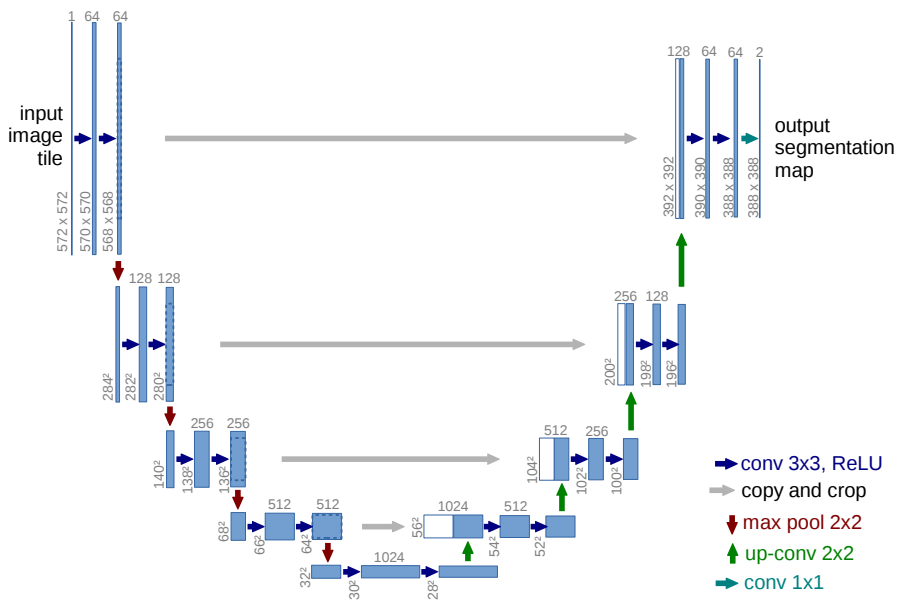
\includegraphics[width=.75\linewidth]{U-NetArchitecture.png} 
	\caption{U-Net architecture taken from~\cite{U-Net} with an contractive path on the left and an expansive path on the right.}
	\label{fig:U-NetArchitecture}
\end{figure}

\subsubsection{Autoencoders} \label{SubSubSec:Autoencoders}
An autoencoder (AE) is a type of CNNs that learns to reconstruct an image from its input without supervision. AEs usually consists of an encoder which extracts the input features, which are stored a low-dimensional latent state space, similar to a U-Net, and a decoder which restore the original input from the latent space. To prevent an AE from learning an identity function, regularized autoencoders were invented, which can be used for e.g. denoising AEs. Variational AEs (VAEs) are generative models that learn latent representation using a variational approach, which constrains the variability of the outputs. VAEs can been used for anomaly detection and image generation~\cite{Fu2020}.

\subsubsection{Generative Adversarial Networks} \label{SubSubSec:GANs}
Generative adversarial networks (GANs) consist of two competing networks, a generator and a discriminator. The generator is trained to generate artificial data that approximate a target data distribution from a low-dimensional latent space similar to an AE. The discriminator is trained to distinguish the artificial data from actual data. The discriminator encourages the generator to predict realistic data by penalizing unrealistic predictions via learning. Therefore, the discriminative loss could be considered as a dynamic network-based loss term. The generator and discriminator both are getting better during training to reach Nash equilibrium. In medical imaging, GANs have been used to perform image synthesis for inter- or intra-modality, such as MRI to synthetic CT and vise versa. In medical image registration, GANs are usually used to either provide additional regularization or translate multi-modal registration to uni-modal registration~\cite{Fu2020}.

\subsection{Deep Learning for Image Registration} \label{SubSec:DLImageRegistration}
Recently, there has been a surge in the use of deep learning based approaches for medical image registration. Their success is largely due to their ability to perform fast inference, and the flexibility to leverage auxiliary information such as anatomical masks as part of the training process. The most effective methods, such as \emph{VoxelMorph}~\cite{Voxelmorph}, typically employ a U-Net style architecture to estimate dense spatial deformation fields. These methods require only one forward pass during inference, making them orders of magnitude faster than traditional iterative methods. Following the success of \emph{VoxelMorph}, numerous deep neural networks have been proposed for various registration tasks~\cite{Fourier-Net+}. Other approaches also utilize CNNs, AEs and GANs. Typical strategies are discussed in more detail in the following sections.

\subsubsection{Supervised Registration} \label{SubSubSec:SupervisedRegistration}
Supervised registration describes training a network with a ground truth displacement field that is either real (created by hand) or synthetic (generated via traditional iterative registration algorithms). Thus the loss can easily be calculated as the difference in the displacement fields of the network prediction and the ground truth (see Figure~\ref{fig:SupervisedRegistration} for a visual overview). These methods have achieved notable results with real displacement fields as supervision. However, this approach is very limited by the size and the diversity of the dataset. As the displacement fields are often calculated by conventional algorithms their effectiveness might be limited for difficult problems with which the traditional algorithms struggle. Fully supervised methods are widely studied and have notable results, but the generation of real or synthetic displacement fields is hard, and these displacements fields might be different from the real ground truth, which can impact the accuracy and efficiency of these kinds of methods~\cite{Zou2022}. Notable approaches include \emph{BIRNet}~\cite{BIRNet} and \emph{LAPNet}~\cite{LAPNet}, however the latter works in the k-space domain.

\begin{figure}[h] %tpb
	\centering
	\graphicspath{{images/}{\main/images/}}
	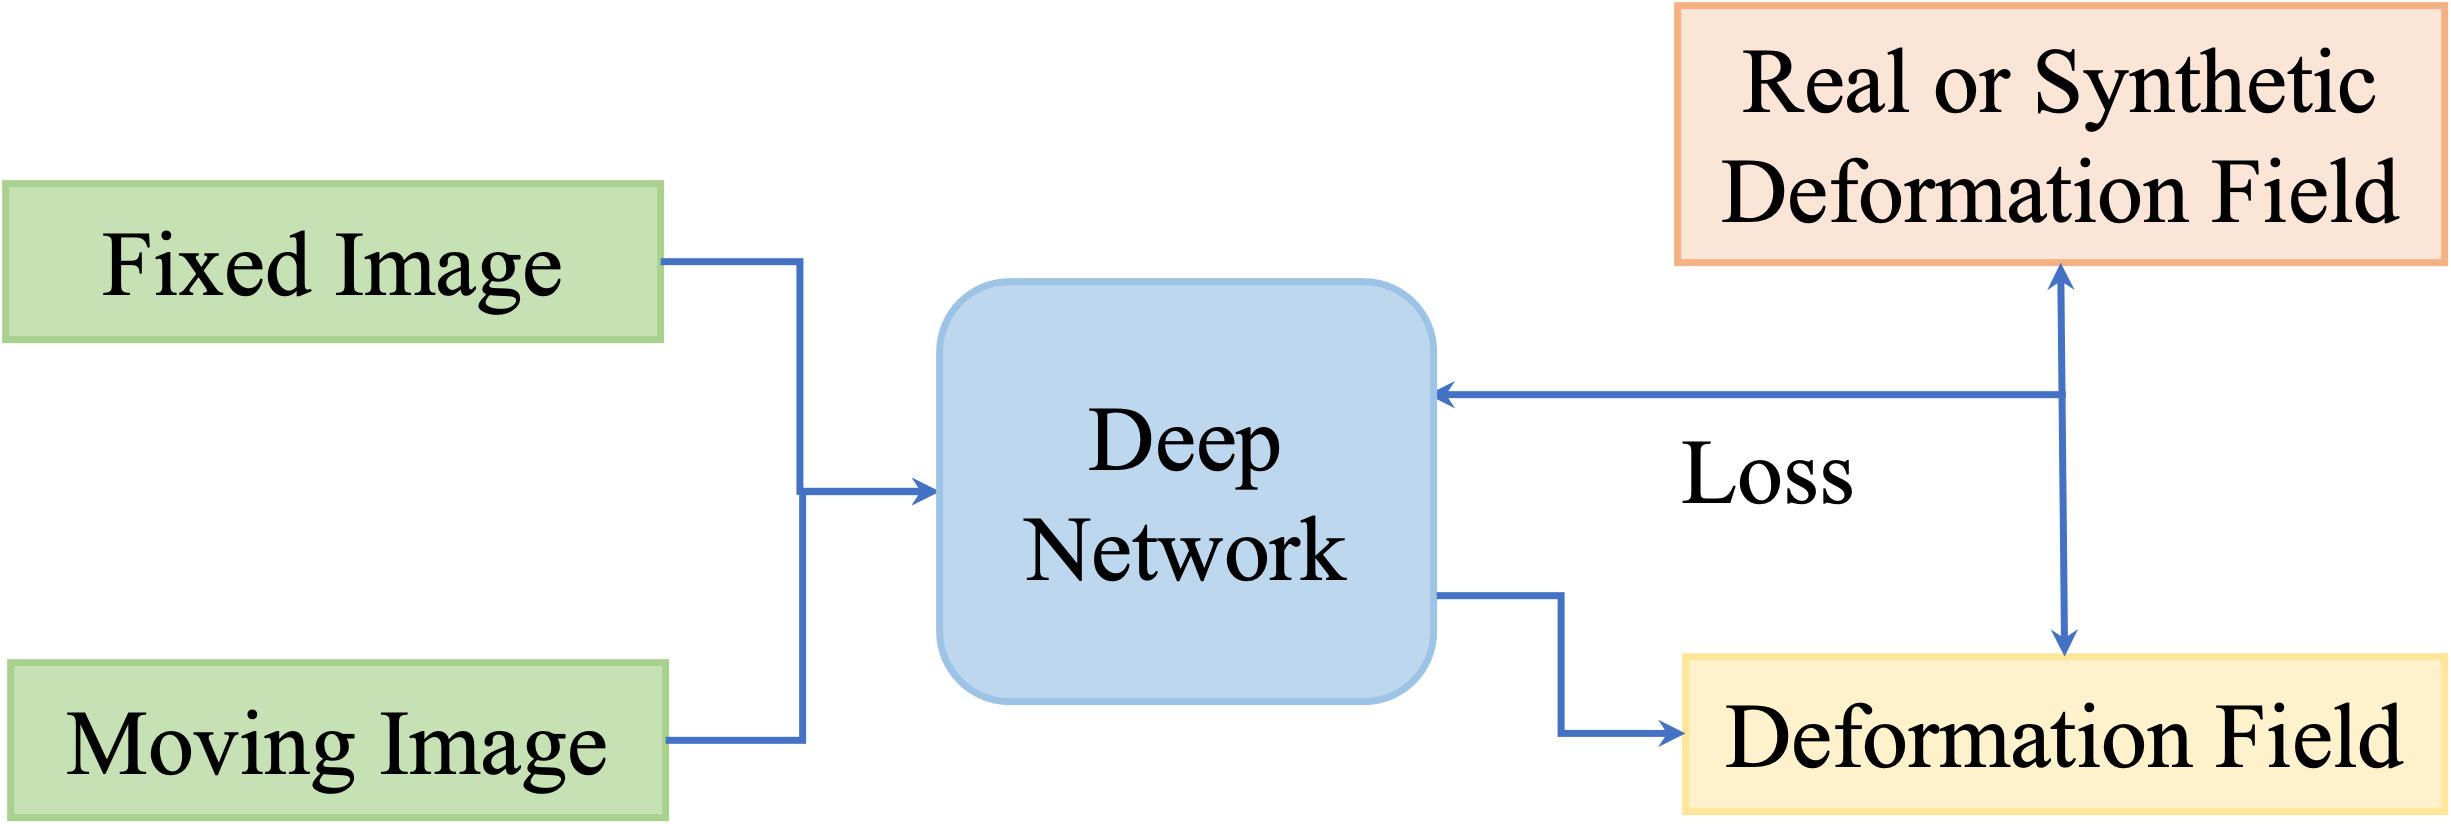
\includegraphics[width=\linewidth]{SupervisedRegistrationGraph.jpg} 
	\caption{Example graph illustrating the training process of a supervised network, taken from~\cite{Zou2022}.}
	\label{fig:SupervisedRegistration}
\end{figure}


\subsubsection{Unsupervised Registration} \label{SubSubSec:UnsupervisedRegistration}
As the preparation of the ground truth displacement field for supervised methods is inconvenient, limitations in generalizing results in different domains and various registration tasks are inevitable. Thus, unsupervised registration has a more convenient training process with paired images as inputs, but without a ground truth. Generally, unsupervised learning consists of similarity-based (see Figure~\ref{fig:UnsupervisedRegistration}) and GAN-based methods (see Figure~\ref{fig:GANRegistration}), where the loss function computes the similarity between the aligned images and the smoothness of the displacement field, rather than the difference to a ground truth~\cite{Zou2022}. Well known example are \emph{IC-Net}~\cite{IC-Net},  \emph{VoxelMorph}~\cite{Voxelmorph}, \emph{TransMorph}~\cite{TransMorph} and \emph{SYMNet}~\cite{SYM-Net}.

\begin{figure}[h] %tpb
	\centering
	\graphicspath{{images/}{\main/images/}}
	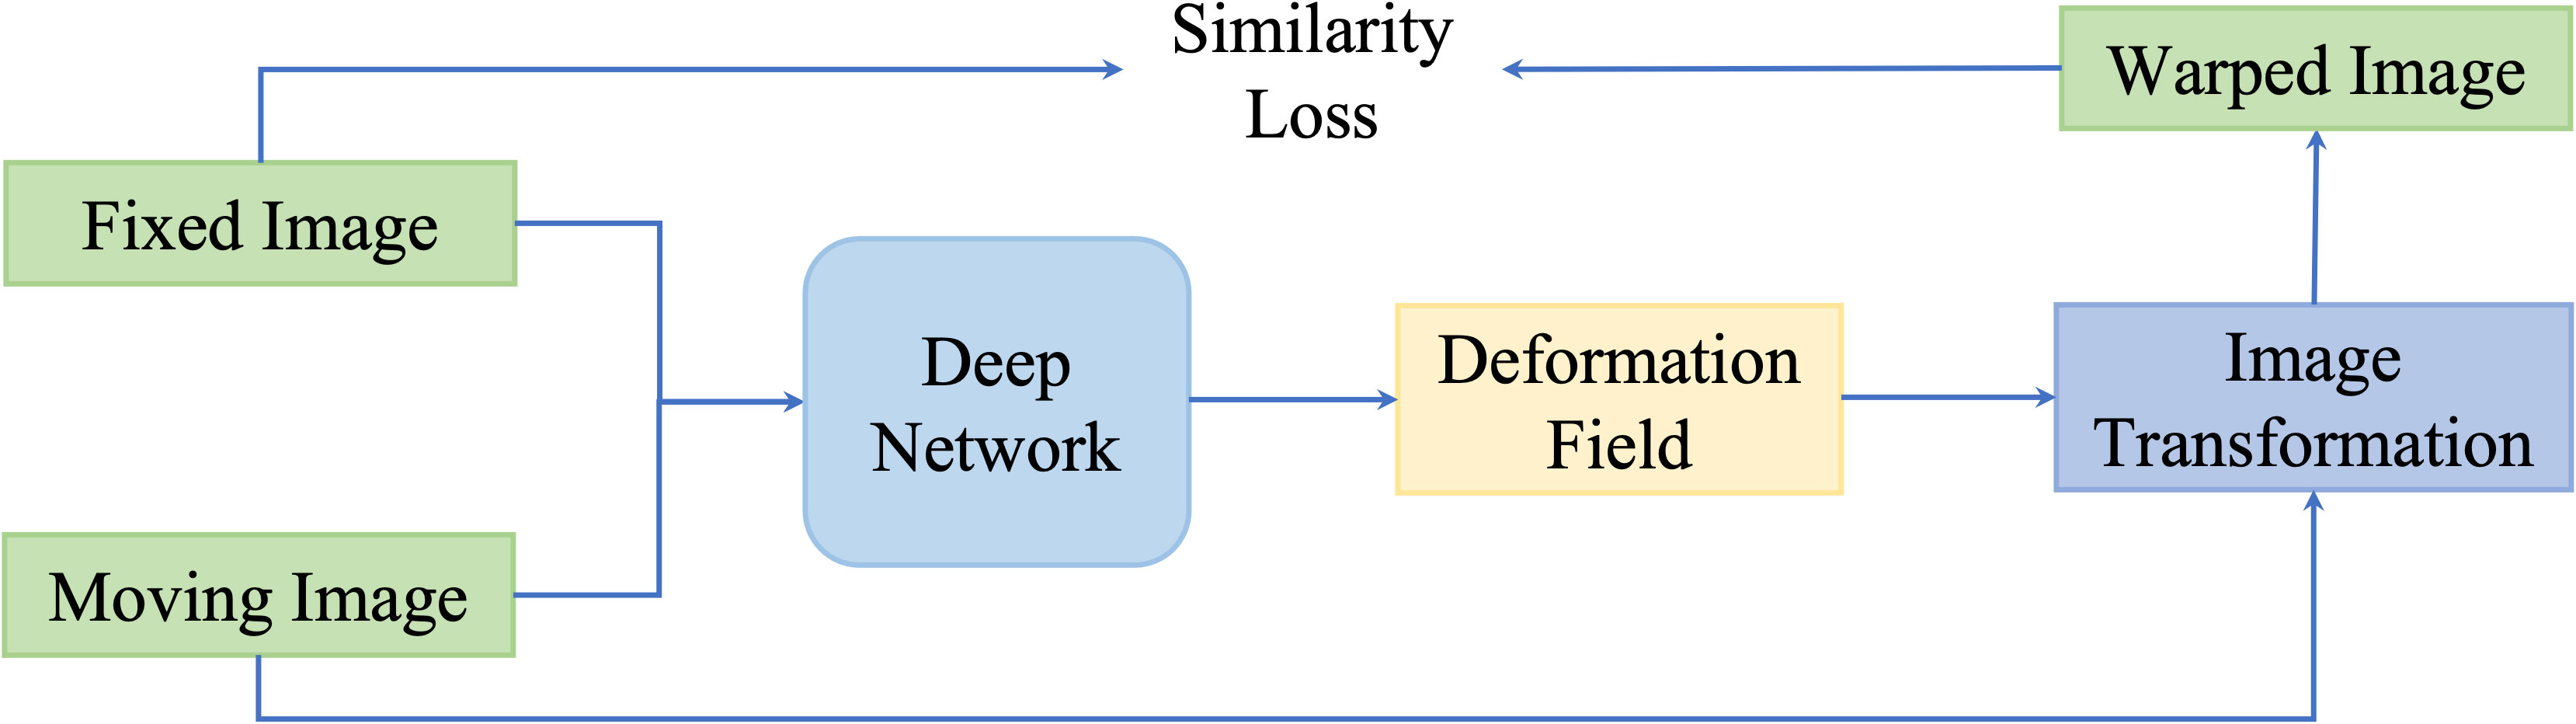
\includegraphics[width=\linewidth]{UnsupervisedRegistrationGraph.jpg} 
	\caption{Example graph illustrating the training process of an unsupervised network with only a image similarity loss, taken from~\cite{Zou2022}.}
	\label{fig:UnsupervisedRegistration}
\end{figure}

\begin{figure}[h] %tpb
	\centering
	\graphicspath{{images/}{\main/images/}}
	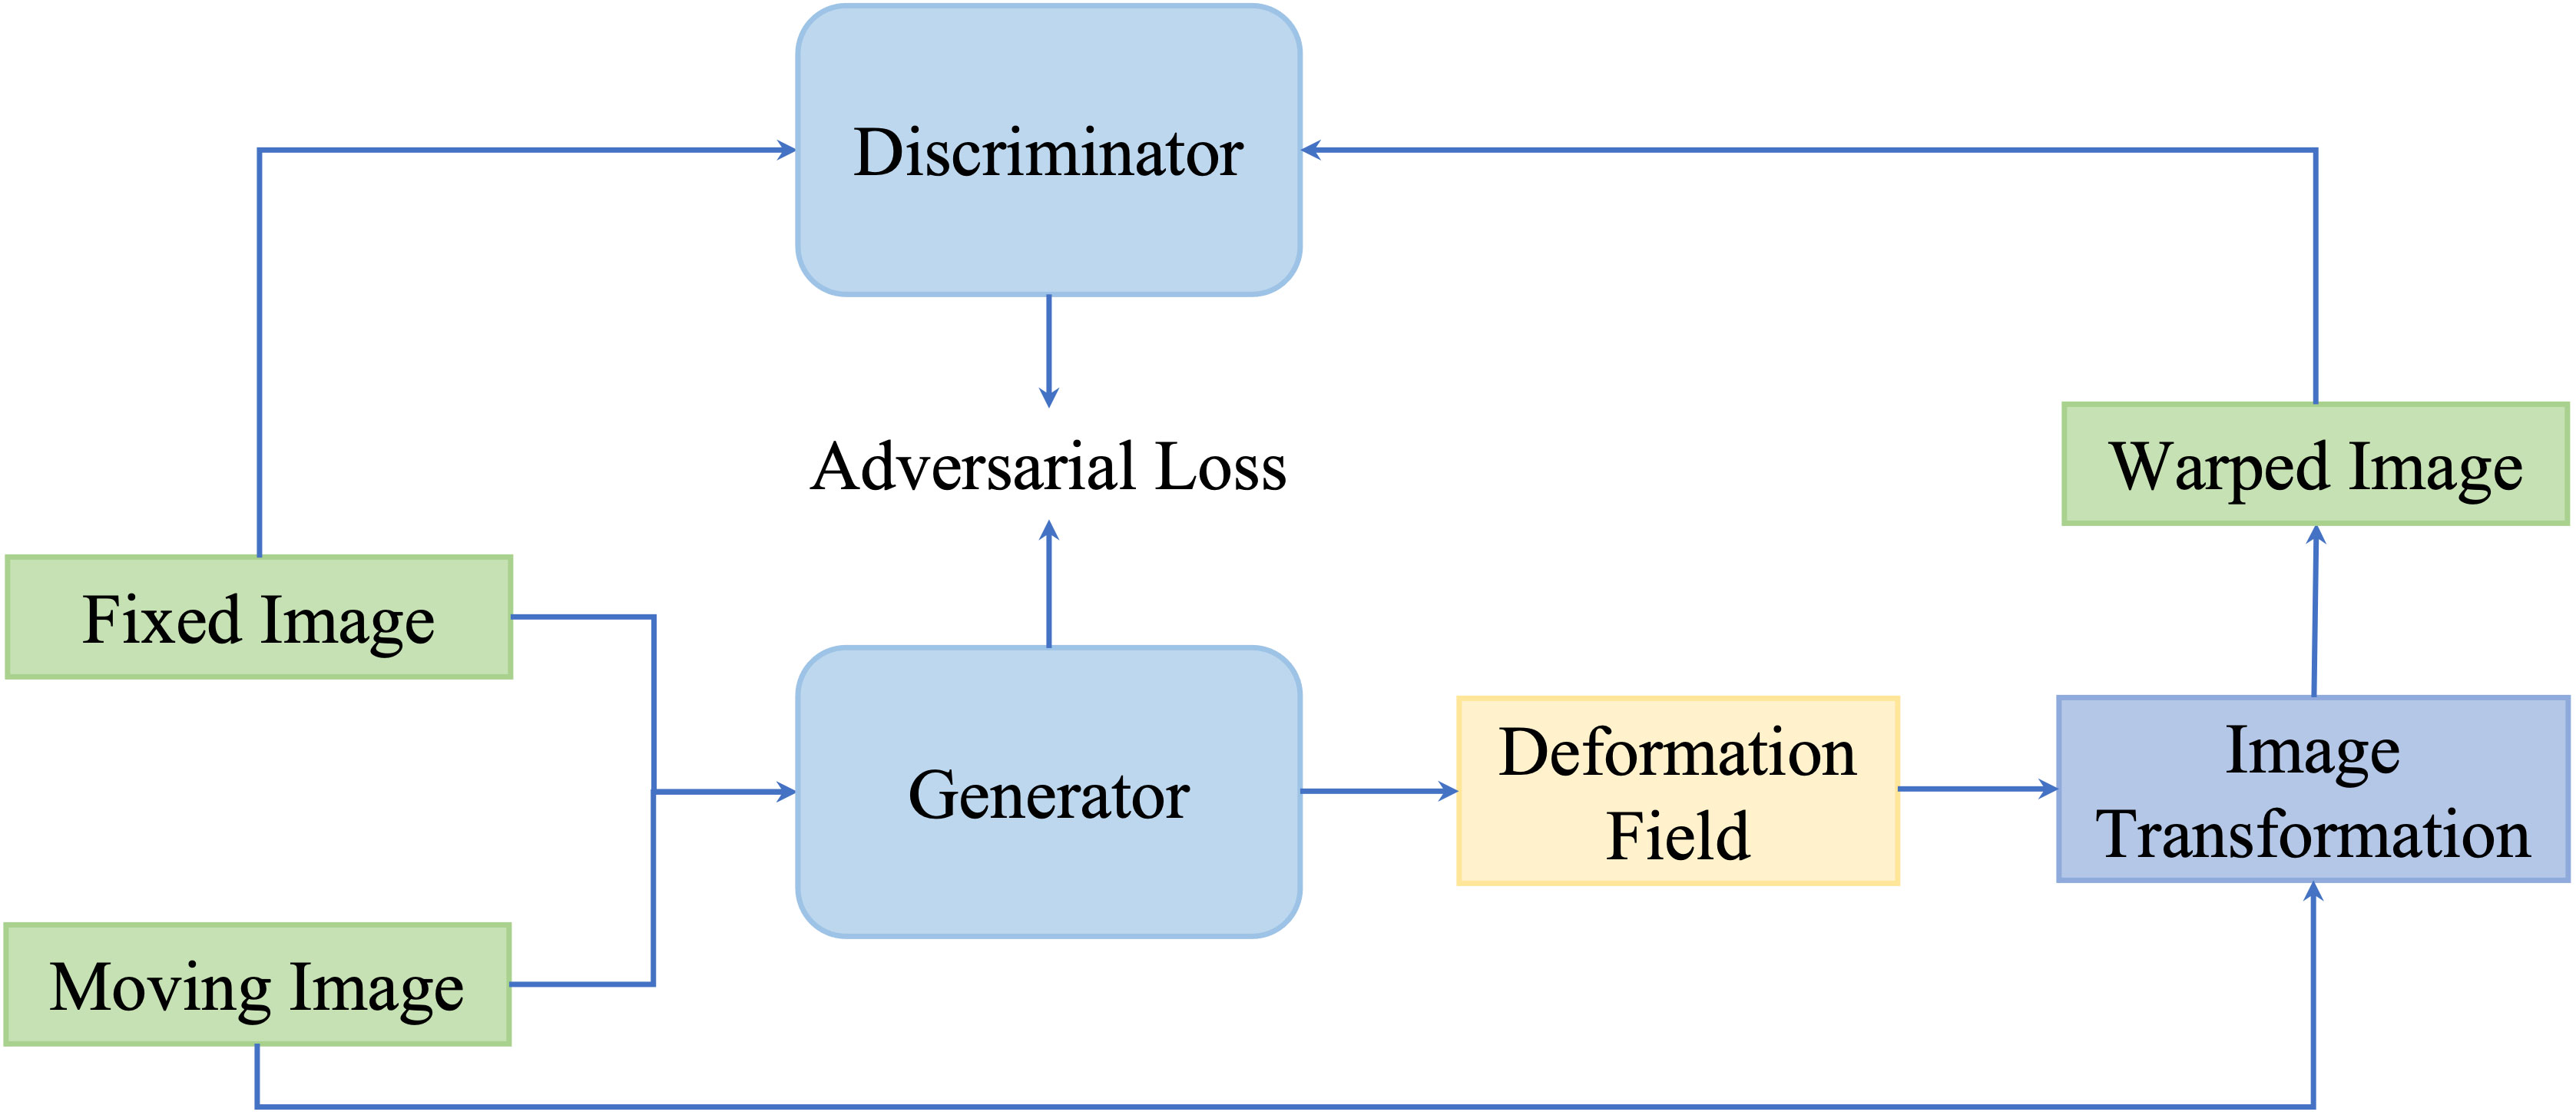
\includegraphics[width=\linewidth]{GANRegistrationGraph.jpg} 
	\caption{Example graph illustrating the training process of a GAN, taken from~\cite{Zou2022}.}
	\label{fig:GANRegistration}
\end{figure}

\subsection{Network Training and Testing} \label{SubSec:NetworkTrainingAndTesting}
In order to train any neural network, a large amount of data is needed. This data can take many forms such as videos, images, audio, text and many more. However, the total data set is usually devided into three subsets: the training, validation and testing subset. 

\subsubsection{Training and Back-Propagation}
The first subset is used for, as the name suggests, the training of the network. This if often the largest of the subsets and should include at lot of variance for the network to learn well. Neural networks in general learn by adapting their weights to perform on increasingly better at a specific task and on a specific dataset/domain. This is done in a process called back-propagation, where the loss calculated between the current output of the model, which is acquired by a simple forward pass through the network, and the desired output is propagated backwards through the model and the weights are optimized using e.g. gradiant decent or similar methods. \\
The second subsets is also used during the training, but is not learned, i.e. no back-propagation is performed. This is done to validate the networks training process and to prevent potential overfitting. Overfitting is a common problem, especially for larger networks, where the network learns every example from the training set, but no general properties as intended. To prevent this, the unseen validation data can be repeatedly used, as it is not learned by the network, to see whether the network improves on unseen data. Once it has been trained for a long time and the validation performance stagnates, or in the worst case even drops, the training process can be stopped. This is known as early stopping and is a very common strategy to prevent overfitting while optimizing training time.\\

\subsubsection{Testing and Evaluation Metrics} \label{SubSubSec:TestingEvalutionMetrics}
The last subset is the testing set, which is used for the final evaluation of the models performance. These usually include tests for the networks performance, as well as memory consumption and inference/execution time. It is important that the test set has not been used for training and is completely unseen by the network. This may sound trivial, but for datasets with a lot of patients providing data all of the data of the patient should be withheld for the testing, which can easily be overlooked.\\
Different metrics can be used for evaluation of a networks registration performance including similarity metrics computed on the images as well as properties of the generated displacement fields. \\
The mean squared error (MSE) is calculated between a fixed (ground truth) image and the warped image giving a pixel-wise comparison:
\begin{equation}
	\text{MSE} = \frac{1}{N} \sum_{i=1}^{N} |F(x,y) - W(x,y)|^2,
\end{equation}
where $F$ is the fixed image and $W$ is the warped image with $N$ being the number of pixels in the images. The lower the MSE the higher the similarity with 0 being a perfect match (the images are exactly the same).\\
The MSE can also be used to calculate another useful metric - the preak SNR (PSNR), which describes the ratio between the maximum possible power of a signal and the power of corrupting noise. It is defined as:
\begin{equation}
	\text{PSNR} = 20 \cdot \log_{10} \bigg(\frac{2^B - 1}{\sqrt{\text{MSE}}} \bigg),
\end{equation}
with $B$ being the bit depth of the image and the metric being defined in decibel (dB) due to the logarithmic scale.\\
%Another common image metric is the normalized cross-correlation (NCC). 
%\begin{equation}
%	\text{NCC} = \frac{1}{N} \sum_{i=1}^{N} \frac{1}{\sigma_F \cdot \sigma_W} F(x,y) \cdot W(x,y),
%\end{equation}
%with image $F$ and $W$ as well as $N$ being the number of pixels in the images. \\
Another common image metric is the structural similarity index measure (SSIM), which operates between 1 (complete similarity) and 0 (no similarity) and tries to estimate the general similarity instead of a pixel-wise comparison making it more robust against contrast changes compared to e.g. MSE.
\begin{equation}
	\text{SSIM} = \frac{(2 \mu_F \mu_W + c_1) \cdot (2 \sigma_{FW} + c_2)}{(\mu_F^2 + \mu_W^2 + c_1) \cdot (\sigma_F^2 + \sigma_W^2 + c_2) },
\end{equation}
where $\mu_F, \mu_W$ are the mean values of the images $F$ and $W$; $\sigma_F^2, \sigma_W^2$ the variances of $F$ and $W$ as well as $\sigma_{FW}$ the covariance for $F$ and $W$, with $c_1, c_2$ being constants derived from the dynamic range of the images. \\
All of these metrics can also be used as loss functions for network training.\\
For comparison of segmentations the Dice score is a commonly used metric to estimate the similarity of two segmentations. A score of 1 indicates a complete overlap/match and a score of 0 indicates no overlapping of the segmentations. The Dice score is calculated as follows:
\begin{equation}
	\text{Dice} = \frac{2 |M_F \cap M_W|}{|M_F| + |M_W|},
\end{equation}
with $M_F$ and $M_W$ being segmentations corresponding to $F$ and $W$ with $M_F$ being a manual segmentation which is warped to obtain $M_W$~\cite{NiftiReg}.\\
Aside from image similarity measures and the evaluation of image segmentations, the displacement field itself can also be evaluated. This is usually based on the assumption that the displacement should be smooth as, for example, folding the image could result in physically unrealistic anatomic structures, indicating errors. Jacobian matrices are the derivatives of the displacement field $\phi$ that form a second order tensor field:
\begin{equation}
	J_{\phi}(p) = \nabla \mathbb{\phi} (p) = \begin{pmatrix}
	\frac{\partial \phi_1(p)}{\partial x_1} & \frac{\partial \phi_1(p)}{\partial x_2} & \frac{\partial \phi_1(p)}{\partial x_3} \\
	\frac{\partial \phi_2(p)}{\partial x_1} & \frac{\partial \phi_2(p)}{\partial x_2} & \frac{\partial \phi_2(p)}{\partial x_3} \\
	\frac{\partial \phi_3(p)}{\partial x_1} & \frac{\partial \phi_3(p)}{\partial x_2} & \frac{\partial \phi_3(p)}{\partial x_3} 
	\end{pmatrix},
\end{equation}
for a point $p$ and encode the local stretching, shearing and rotating of the displacement field. The determinants of such matrices, also called the Jacobian determinants of the deformation $|J_{\phi}|$, must be positive everywhere to avoid folding as a region of negative determinants would indicate that the one-to-one mapping has been lost~\cite{DARTEL}. Thus the percentage of non-positive Jacobian determinants of the deformation $\% \, |J_{\phi}|\leq0$ can be used to evaluate the quality of the generated displacement field~\cite{Chen2023}.
